\documentclass[a4paper]{article}

\usepackage{linguex}
\usepackage{caption}
\usepackage{graphicx}
\usepackage{fixltx2e}
\usepackage{comment}
\usepackage{hyperref}
\usepackage{endnotes}
\usepackage{natbib}
\usepackage{epstopdf}

\bibliographystyle{apalike}
\graphicspath{ {Figures/} }

\title{Knowledge \textit{wh} and False Beliefs:\\Experimental Investigations}

\author{Jonathan Phillips \& B. R. George}

\begin{document}

\maketitle


\begin{abstract}A common approach to knowledge \textit{wh} is to try to reduce it to knowledge \textit{that}, and in particular to answer-knowledge. On this view, the truth-conditions of a knowledge \textit{wh} ascription can be given entirely in terms of which answers to the embedded question the subject knows. Against this background, this paper considers the phenomenon of \emph{false-belief sensitivity} --- a challenge to this common approach to knowledge \textit{wh} that has recently received a fair amount of attention in the question embedding literature. We present a series of experiments that help to bring the empirical standing of this phenomenon into focus. Across six experiments, our results provide evidence that truth judgments of knowledge \textit{wh} ascriptions are affected by both the presence of false beliefs and the proportion of the subject's beliefs that are false. Collectively, these results demonstrate a pattern of judgments that is incompatible with standard accounts of the relationship between knowledge \textit{that} and knowledge \textit{wh}, and with reducibility more generally. After presenting these new data, we end by considering the theoretical implications of this richer descriptive picture and outline a number of remaining open questions that should be pursued in future work.\\

\noindent \textbf{keywords}: knowledge \textit{wh}; false belief; embedded questions; knowledge \textit{that}
\end{abstract}


\section{\textit{knowing wh} and \textit{knowing that}}

In linguistic and philosophical work on question-knowledge ascriptions, a common point of departure is the assumption that knowledge \textit{wh} admits straightforward description in terms of knowledge \textit{that}. On this view, the truth-conditions of a knowledge \textit{wh} ascription can be given entirely in terms of what answers to the embedded question the subject knows. With a few notable exceptions, the mainstream approach has been to assign \ref{jknowswherealpha} truth-conditions equivalent to those given by \ref{paraphrase}, for some understanding of what it is to ``answer'' or ``resolve'' a question:\footnote{Exactly what constitutes answering or resolving a question is theory-dependent and may be contentious, and choices in this area provide some flexibility within the general approach outlined here.}

\ex.\label{jknowswherealpha}\label{sueknows}Sue knows where she can buy an Italian newspaper.

\ex.\label{paraphrase}$\exists p$ s.t.\ $p$ answers/resolves ``Where can S.\ buy an Italian newspaper?'' and S knows $p$.

Influential approaches to knowledge \textit{wh} that can be framed in terms of \ref{paraphrase} include those of \citet{karttunen:77}, \citet{gs:84}, \citet{br:99}, and \citet{lahiri:02}.\footnote{When we say they can be framed in these terms, we mean that their predicted truth-conditions for sentences like \ref{jknowswherealpha} can be restated as in \ref{paraphrase}, so that \ref{paraphrase} captures a logical dependency between knowledge \textit{wh} an knowledge \textit{that}. This need not involve knowledge \textit{that} being more primitive than knowledge \textit{wh} in some specific theoretical sense --- indeed, the authors cited differ significantly in how they formalize the relationship between instances of \textit{know} in the two ascription types.} A possible general principle analogous to the presentation in \ref{paraphrase} is discussed by \citet{higginbotham:96}. On this picture, the truth of knowledge \textit{wh} ascriptions is sensitive to no propositional attitudes of the subject other than knowledge \textit{that}, and is concerned only with \emph{true} answers to the embedded question.\footnote{The truth requirement is not explicit in \ref{paraphrase}, but falls out from the fact that knowledge is factive. Many accounts also build a truth requirement in to their notion of answerhood.}


This paper is concerned with \emph{false-belief sensitivity} --- a challenge to this picture that has recently received a fair amount of attention in the question embedding literature. We present a series of experiments that help to clarify the empirical picture of this phenomenon.

\subsection{False Belief Sensitivity: Empirical Issues}

The issue we take up can be seen by considering the following sentences (adapted from \citet{george:dis}). Reported judgments suggest that the truth of \ref{jknowswherealpha} depends on the truth or falsity not just of ascriptions-of-true-knowledge like \ref{trueknow1intro} and \ref{trueknow2intro} but also on the truth or falsity ascriptions-of-false-belief like \ref{falsebel1intro}:

\ex.[\ref{jknowswherealpha}]\label{sknwha} Sue knows where she can buy an Italian newspaper.


\ex. \a.\label{trueknow1intro}Sue knows that she can buy a Italian newspaper at Newstopia.
\b.\label{trueknow2intro}Sue knows that she can't buy an Italian newspaper at PaperWorld.
\c.\label{falsebel1intro}Sue believes (incorrectly) that she can buy an Italian newspaper at PaperWorld.

To make this challenge clearer, consider the two vignettes \textbf{All True} and \textbf{Mixed}. In the \textbf{All True}, Newstopia sells Italian Newspapers and Paperworld doesn't, and Sue knows Newstopia sells Italian newspapers (i.e., \ref{trueknow1intro} is true) but has no beliefs one way or the other about PaperWorld (i.e., neither \ref{trueknow2intro} nor \ref{falsebel1intro} is true). Vignette \ref{bobright1} gives a natural description of an \textbf{All True} situation. In \textbf{All True}, the relatively uncontroversial judgment is that \ref{jknowswherealpha} is true.

\ex.\label{bobright1}(\textbf{All True}) Sue is standing on the street near a store called Newstopia. Sue's friend, Bob, a native of the city who is normally very well-informed and trustworthy, told her that she can buy an Italian newspaper at Newstopia. Having no reason to doubt this, Sue took Bob at his word. Bob was correct about Newstopia, which does sell Italian newspapers.

In a \textbf{Mixed} vignette, by contrast, Sue again knows that Newstopia sells Italian newspapers, but she further believes (erroneously) that PaperWorld does as well, so both \ref{trueknow1intro} and \ref{falsebel1intro} are true. Vignette \ref{bobwrong1} gives  more natural example of this case. In this scenario, the (more contentious) reported judgment is that \ref{jknowswherealpha} is untrue.\footnote{For these cases, the relevant judgments are discussed by \citet{george:dis,george:thought,cremers:plurality,theiler:etal,xiang:sub:16}.}

\ex.\label{bobwrong1}(\textbf{Mixed}) Sue is standing on the street near two stores: one called PaperWorld, and another called Newstopia. Sue's friend, Bob, a native of the city who is normally very well-informed and trustworthy, told her that she can buy an Italian newspaper at PaperWorld, and also at Newstopia. Having no reason to doubt this, Sue took Bob at his word. However, Bob completely misinformed Sue about PaperWorld, which does not sell newspapers, but actually just sells stationery and office supplies. Bob was correct about Newstopia.

If both of these judgments are as described, then it suggests that holding Sue's answer-knowledge fixed while varying her false beliefs can change the truth of the knowledge \textit{wh} ascription. This type of sensitivity is plausibly incompatible with a family of approaches informally illustrated by \ref{paraphrase}.\footnote{The reader may have noticed a similarity between these examples and the well-known strongly exhaustive readings of embedded questions. There is an obvious similarity, and many authors (e.g., \citet{kr:11}, \citet{cremers:plurality}, and \citet{theiler:etal}, among others) have attempted to provide unified theories accounting for both false-answer sensitivity and strong exhaustivity. However, the two phenomena are descriptively distinct, as discussed by, e.g., \citet{george:dis}, \citet{cremerschemla:2014}, and \citet{theiler:etal}. Roughly, strongly exhaustive readings involve a different notion of answer - one that involves both positive and negative information, but are still able to resolve things in terms of what true answering information is known. In contrast, false-belief sensitivity distinguishes between cases where a person doesn't know negative information because they have formed no opinion on the matter, and cases where they don't know it because they have beliefs that contradict it.}

The possibility of false-belief sensitivity with knowledge \textit{wh} has been discussed in a number of settings: it is entertained by \citet{gs:82} (who reject it) and \citet{berman} (who excludes it from the semantics (narrowly construed), but tries to derive something like it with a classically Gricean conversational implicature approach. A semantics that incorporates it is explicitly advocated by \citet{spector:05}. More recently, it has received renewed attention from, among others, \citet{kr:11}, \citet{george:dis, george:thought}, \citet{cremerschemla:2014}, \citet{cremers:plurality}, \citet{theiler:etal} and \citet{xiang:sub:16}, who have introduced a variety of different theoretical approaches.

\subsubsection{Our Empirical Contribution} 

As suggested by the growing attention paid to this issue, judgments related to false-belief sensitivity are theoretically interesting for a variety of reasons. Yet, there remains a lack of clarity about the introspective judgments that are meant to provide support for false-belief sensitivity. This is the main motivation for our systematic experimental investigation.

All of our experiments are concerned with false-belief sensitivity for \emph{mention-some} readings of embedded questions, like the salient readings of our ``Italian newspaper'' examples above. In these readings, the question is intuitively resolved by providing a single instance of something that can ``fill in'' for the \textit{wh} expression, in contrast with \emph{mention-all} readings, where resolving the question involves some kind of complete information. Mention-some readings of embedded questions have been recognized for quite some time, but false-belief sensitivity with such readings has received sustained attention only relatively recently. For examples of recent work, see \citep{george:dis,cremerschemla:2014,theiler:etal,xiang:sub:16}.

We will not explore mention-all readings, which have been discussed in connection with false-answer sensitivity for considerably longer. This is the type of false-answer sensitivity discussed by \citet{gs:82}, \citet{berman}, and \citet{spector:05}. Such a possible reading has continued to receive theoretical attention (e.g. \citet{theiler:etal} \citet{xiang:sub:16}, \citet{cremers:plurality}), and is investigated experimentally by \citet{cremerschemla:2014}, who report empirical evidence for the availability of such a  reading. It is important to explore the possibility of false-belief sensitivity of both the mention-some and mention-all types, as theories differ on the relationship between mention-all and mention-some readings, and an account of a false-belief effect for one will not necessarily carry over to the other.

We investigate a number of different aspects of judgments of knowledge \textit{wh} ascriptions, but one important topic that is worth highlighting at the outset is the prospect of \emph{proportion-sensitivity} with false-belief effects. It has been our impression in informal discussions with other philosophers and linguists that the contrast in truth judgments between the \textit{All true} and \textit{Mixed} cases is strongest when the agent has a large number of false beliefs (relative to the number of true beliefs), and weakest when these proportions are reversed. We explore this phenomenon directly in our final experiment. This possibility is of particular theoretical interest because it is not derived by current accounts of false-belief sensitivity, which present a more all-or-nothing picture, and has not been explored in extant literature.

\subsection{False Belief Sensitivity: Theoretical Issues}

The false-belief sensitivity effect for knowledge \textit{wh} connects with two broader issues in the semantics of question embedding: it belongs to the wider phenomenon of \emph{false-answer sensitivity}, and it is a challenge to any approach that requires that knowledge \textit{wh} be \emph{reducible} to knowledge \textit{that}.

First, briefly consider the wider problem of \emph{false-answer sensitivity}. A number of embedders are plausibly described as imposing one condition with respect to true answers, and another with respect to false answers. One example occurs with \textit{tell wh}. According to, e.g., \citet{kr:11}, \ref{atoldb} has a reading on which it is true under roughly the conditions given in \ref{atoldblogic}:

\ex. \a.\label{atoldb}Alice told Bob who was at the party.
\b.\label{atoldblogic}$\forall x\left(\begin{array}{l}\textrm{If $x$ was at the party, A told B that $x$ was there}\\\multicolumn{1}{r}{\textrm{\footnotesize (true answer condition)}}\\\textbf{\&}\\\textrm{If $x$ wasn't at the party, A didn't tell B that $x$ was there}\\\multicolumn{1}{r}{\textrm{\footnotesize (false answer condition)}}\end{array}\right)$

This is a departure from the default picture exemplified for by \ref{paraphrase} above (or, rather, from its natural generalization to \textit{tell}). This general sort of false-answer sensitivity has been claimed for \textit{tell}, a variety of other attitudes (cf., e.g., \citet{berman,heim:94,kr:11,preuss}). False-belief sensitivity for knowledge \textit{wh} is thus of interest in part as an instance of this (still incompletely understood) wider issue.


Second, false-belief sensitivity with knowledge \textit{wh} is a challenge not just to the type of picture in \ref{paraphrase} but to any picture where the facts for the knowledge \textit{wh} relation at a given time are fully determined by the facts for the knowledge \textit{that} relation at that time. This feature distinguishes it from the false-answer effect with \textit{tell} in that it presents a potential challenge to the \emph{reducibility} of knowledge \textit{wh} to knowledge \textit{that}, while false-answer sensitivity of \textit{tell} does not pose a similar problem.

Most older treatments of knowledge \textit{wh}, and most attempts at general uniform-across-attitudes accounts of question embedding under propositional attitudes, conform to this reducibility principle, although few explicitly articulate it, and many would reject any role for such a reduction in the grammar. There are, of course, a number of exceptions to this picture, including much of the work on false-belief sensitivity, going back at least to \citet{spector:05}.\footnote{The picture of false-belief sensitivity that \citet{gs:82} entertain would also be non-reducible. Berman's (\citeyear{berman}) account, on the other hand, regards this effect as non-truth-relevant and computed by something like general Gricean mechanisms, so if Berman's picture of the nature and origin of false-belief sensitivity is accurate, reducibility can be maintained.}

The reported false-belief sensitivity for \textit{know} is a problem for reducibility because the difference in truth of \ref{jknowswherealpha} between \textbf{Mixed} and \textbf{All True} depends only on Sue's false beliefs, which are not recoverable from her knowledge (which remains the same across the two vignettes).\footnote{See \citet{george:dis,george:thought} for a more detailed discussion of the problem.} 

In contrast, false-answer effects for \emph{tell}, at least as described above, do not present a similar problem, because the true answer and false answer components for telling \textit{wh} both involve telling \textit{that}, where telling \textit{that} is not veridical (see \citet{kr:11}). Since false belief is not recoverable from knowledge \textit{that}, knowledge presents a reducibility problem that telling does not. There are also reported judgments that support non-reducibility for some attitudes without truth-sensitivity: \textit{agree} is a likely candidate here (see \citet{cg:15}).

The concept of reducibility is explicitly discussed by \citet{kr:11} and \citet{george:dis}. In both cases, reducibility appears to be regarded as a presumptively \emph{desirable} feature of a theory of question embedding, because it gives a clear and potentially uniform story of how the question-embedding and propositional forms of a given embedder are related. Both discussions further note that false-belief sensitivity for \textit{know} is at odds with reducibility (given certain plausible background assumptions).

If reducibility does fail, and if we want any nontrivial general principle connecting the \textit{that} and \textit{wh} forms of the same embedder, we will have to look elsewhere. We are more likely to succeed in articulating and defending an alternative if we have a clear empirical picture of the circumstances under which reducibility fails. This is the aim of the current paper. 

\subsection{Plan of the Paper}

We present six experiments that collectively provide a clearer descriptive picture of the role of false-belief sensitivity in knowledge \textit{wh}. Experiment 1 demonstrates that ordinary truth-value judgments of knowledge \textit{wh} ascriptions are sensitive to the agent's false beliefs. Experiment 2 expands on this basic effect by showing false-belief sensitivity persists across a number of different kinds of \textit{where} question constructions and even for negated knowledge \textit{wh} ascriptions. We then pause to show that this effect is unlikely to be explained by a degradation of the knowledge \textit{that} facts (Experiment 3) or by Gricean relevance implicatures (Experiment 4). In Experiment 5, we go on to offer evidence that this effect extends to a number of different kinds of theoretically interesting knowledge \textit{wh}, including knowledge \textit{who} and knowledge \textit{how}. Finally, in Experiment 6, we demonstrate that ordinary truth-value judgments of knowledge \textit{wh} are sensitive not only to the presence of false belief but to the \textit{proportion} of the agent's beliefs that are true (vs. false). We end by considering the theoretical implications of this richer descriptive picture and outline a number of remaining open questions that should be pursued in future work. 

\section{Experiment 1: An Initial Test} \label{sec:study1}

We began by testing whether ordinary truth assessments reflect the proposed false-answer sensitivity in the type of scenario described in \textbf{All True} and \textbf{Mixed}. The aim of this first experiment was to establish a rough sense of the basic empirical status of the reported intuitions, and the plausibility of the associated non-reducibility claims.

\subsection{Methods} \label{sec:study1Methods} 103 (53 females, age $M(SD) = 34.32(12.11)$) participants with American IP addresses were recruited from Amazon's Mechanical Turk (www.mturk.com) and paid a small amount of money (\$0.20) in compensation for a small amount of their time ($<$ 5 minutes) \citep{buhrmester2011amazon,paolacci2014inside,sprouse2011validation}. Additional demographic information about these participants can be found in the supporting materials. For this study, and all of the following, all stimuli, data, analyses, and other supporting materials can be retrieved from: \url{https://github.com/phillipsjs/Knowledge_wh}

Participants read vignettes \textbf{All True} (in which Sue knows an answer and has only true beliefs) and \textbf{Mixed} (in which Sue knows an answer and has relevant false beliefs) in counterbalanced order. After reading each vignette, participants were asked to indicate their agreement with \ref{sueknows} on a scale from 1 (``Completely disagree'') to 7 (``Completely agree'').

\ex.[\ref{sueknows}]Sue knows where she can buy an Italian newspaper.

Finally, participants were asked to summarize the difference between the two stories and then completed a series of optional demographic items including a question asking whether English was their native language. 

\subsection{Results}

2 participants were excluded because they did not indicate that English was their native language. For simplicity, we first consider only participants' responses on the first trial.\footnote{Throughout, we focus on first-trial results, and conduct only one or two trials per participant. These decisions are motivated by a desire to minimize demand characteristics of the study which could bias participants' responses by causing them to focus on the aspects of the experiment that vary across trials.} In \textbf{All True}, when Sue had only true beliefs about stores that sold Italian newspapers, participants tended to strongly agree with \ref{sueknows} ($M(SD) = 6.23(1.35)$). This is the expected under any analysis that assigns a mention-some reading. However, in \textbf{Mixed}, when Sue had one true and one false belief, participants agreed significantly less with \ref{sueknows} ($M(SD) = 4.88(2.16)$), $t(79.83) = 3.75$, $p < .001$, $d = .757$. This is in line with a false-belief sensitivity story, where \ref{sueknows} is untrue in this case, but (on a mention-some reading) not for accounts that satisfy reducibility.

Additional analyses revealed that this pattern did not change when considering participants' responses to both the first and second trials and was not affected by the order in which participants completed the tasks.\footnote{A paired-samples analysis of participants' responses to both conditions again revealed a difference in participants' agreement ratings in the two conditions $t(100) = 3.94$,  $p < .001$, $d = .529$, and a comparison of linear mixed-effect models \citep{bates2012lme4,jaeger2008categorical,gelman2006data} revealed that there was no main effect of the order in which the items were completed, $\chi^2(1) = 0.17$, $p = .682$, and no Condition $\times$ Order interaction effect, $\chi^2(1) = 2.51$, $p = .113$.}

These patterns can be seen in (Fig. \ref{fig:Fig1}), where we graph the distribution of participants' responses using box plots. In this plot, and in those that follow, individual dots depict participants' responses (the dots were jittered to prevent overlap). The ``hinges'' of the box (the top and bottom lines of the box) depict the 25th and 75th percentiles, and thus to boxes themselves should be understood as a representation of the middle 50\% of the data. The thicker horizontal black bars indicate the median response that participants gave in that condition. While these graphs should help readers get a sense for the entire distribution of participants' responses, the mean rating and variance for the different conditions are also reported in the ``Results'' sections throughout the paper.

\begin{figure}[h!]
\centering
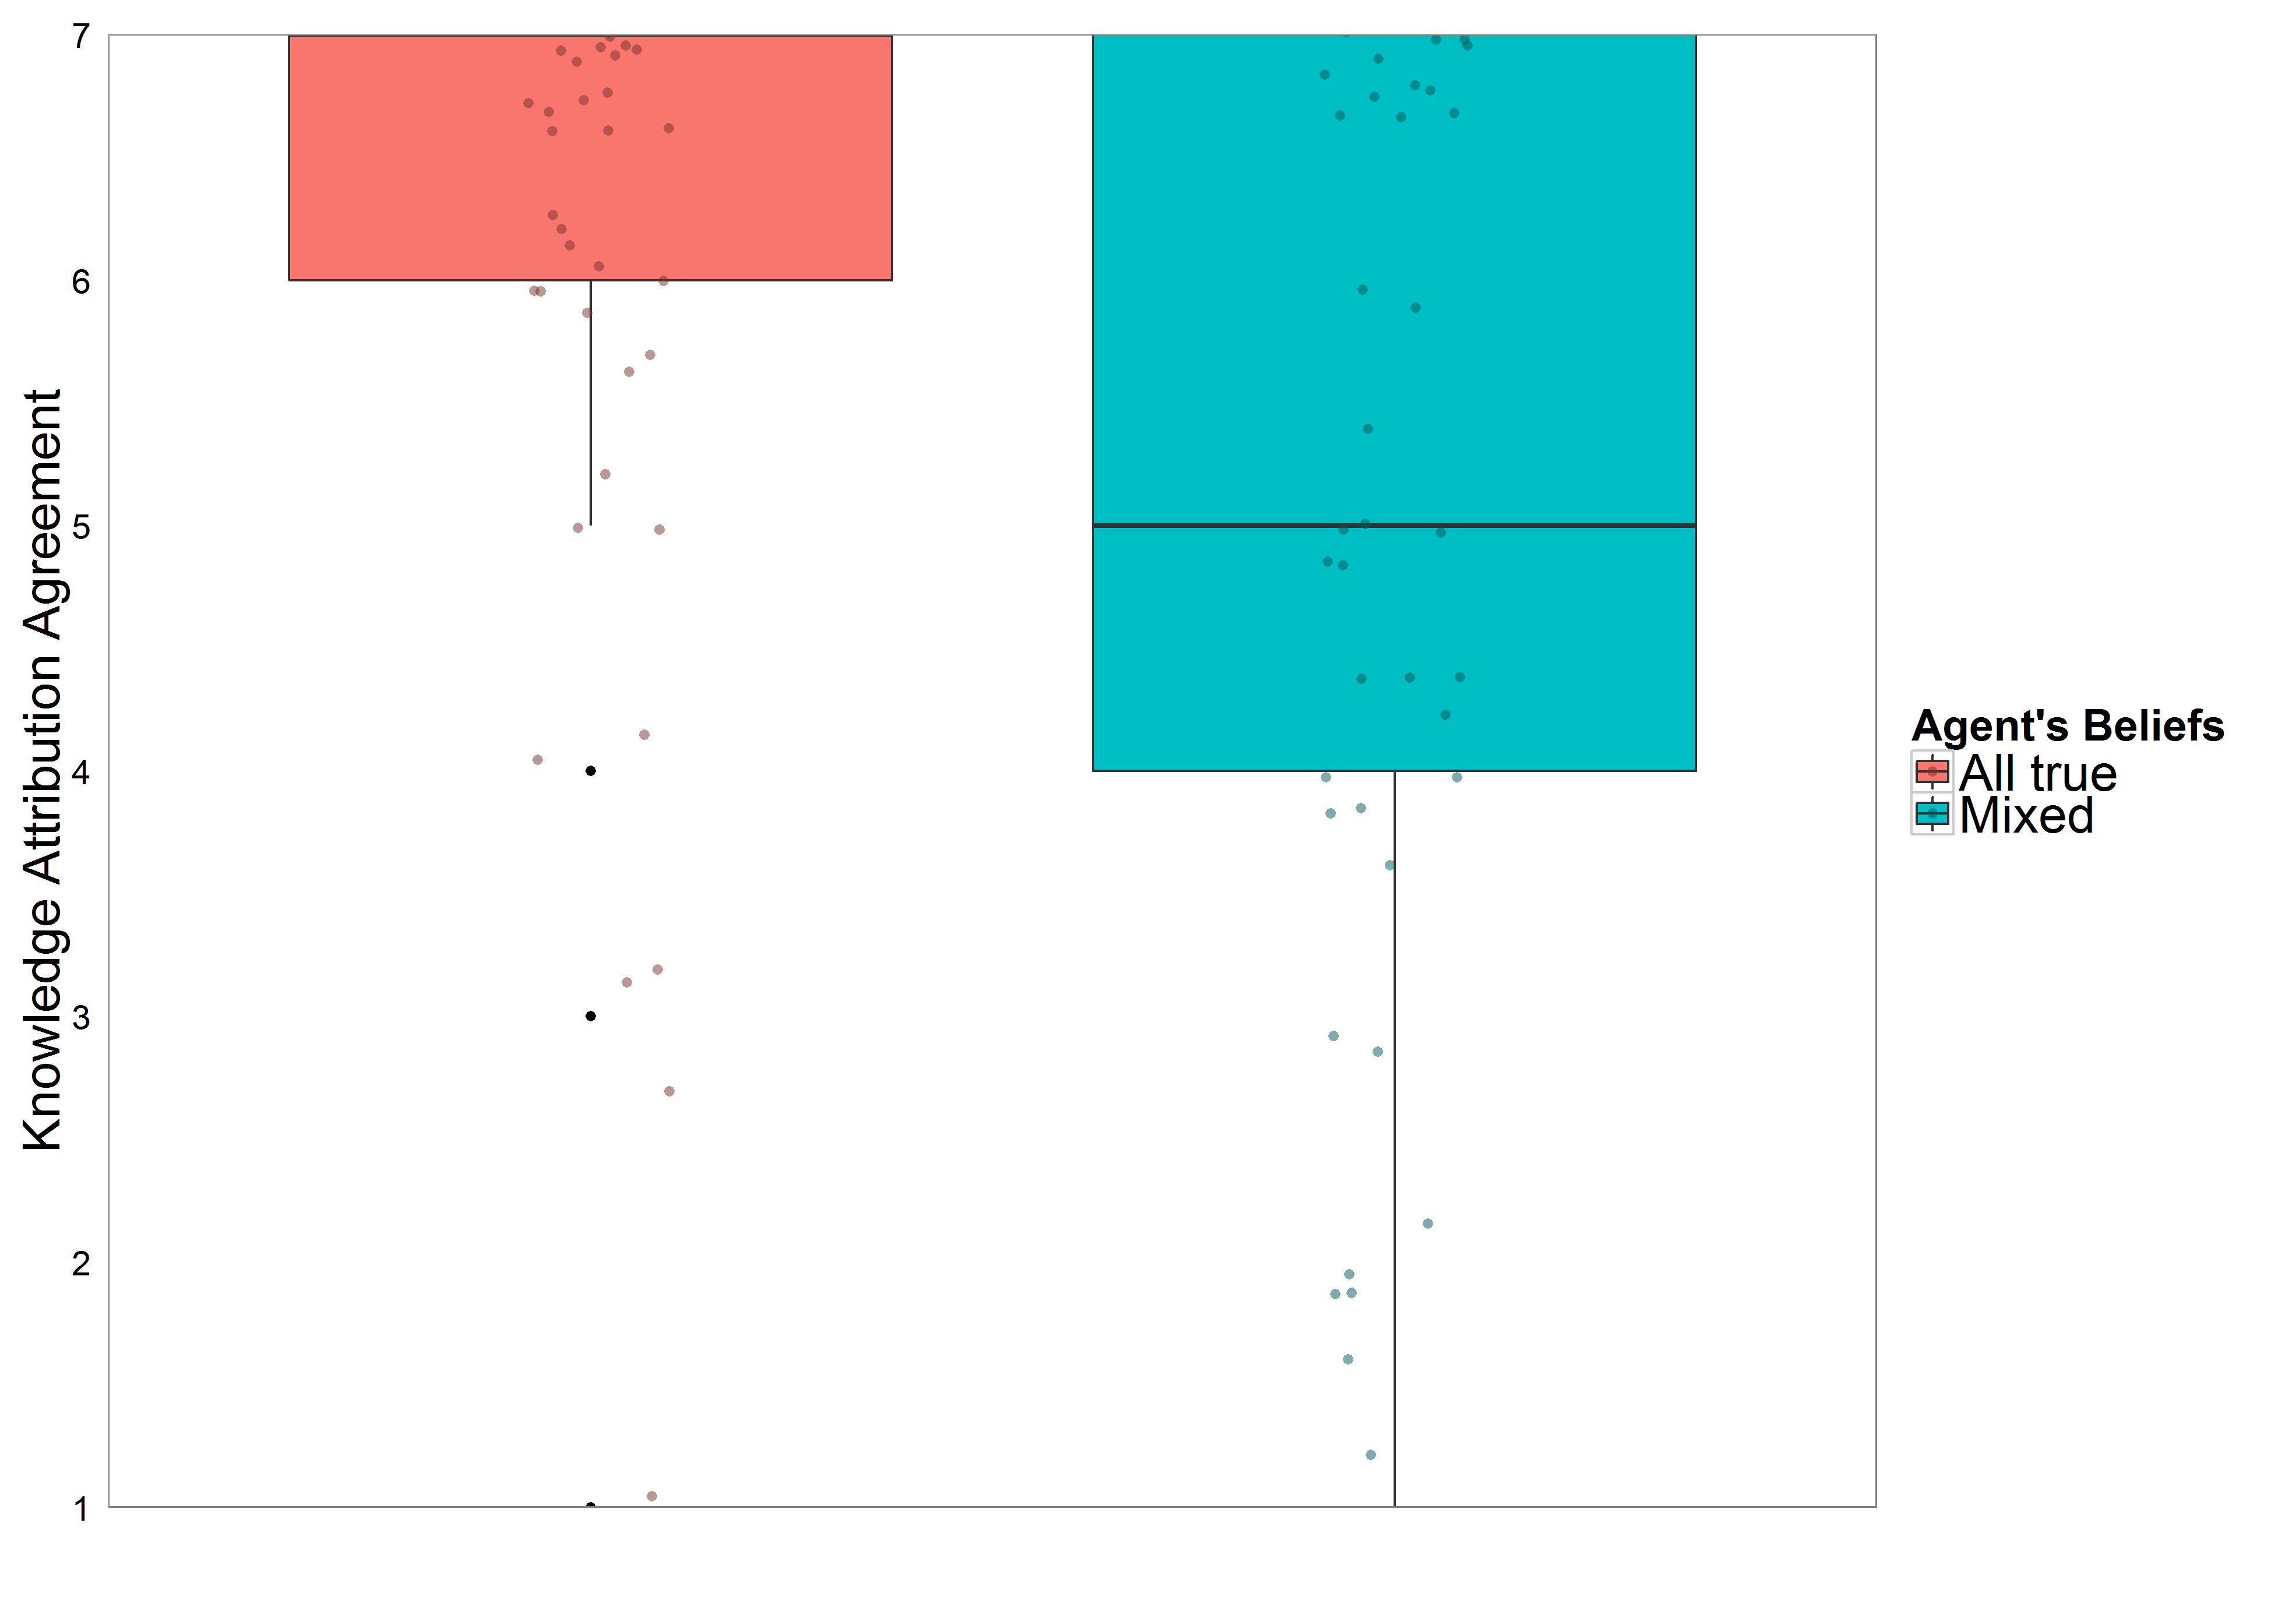
\includegraphics[width=14cm] {Fig1}
\captionsetup{width=0.9\textwidth}
\caption{Boxplots of participants' agreement rating with the knowledge ascription in the \textbf{All true} and \textbf{Mixed} conditions.}
\label{fig:Fig1}
\end{figure}

\subsection{Discussion}
The results of this study provide some initial evidence that native-speaker truth-value judgments align with the false-answer sensitivity claims insofar as speakers distinguish between the truth status of \ref{sueknows} in the cases with and without false beliefs. At the same time, participants' level of agreement also differs from what would be expected for a clear false case. This is not necessarily a problem for a general non-reducibility claim, but it does count against any implementation that predicts false  reliably produce simple at-issue falsehood, without some additional mitigating factor.\footnote{Thus, for example, the implementation of false-answer sensitivity in \cite{george:dis}, which places the ``no false beliefs'' requirement among the core truth conditions, seems like a poor candidate. (Note, though, that George presents this account as preliminary, and indicates that presuppositional possibilities also require consideration.)}

This intermediate agreement rating does not straightforwardly fall out of a simple bivalent truth-conditional account. The question we face is one of whether we have a false-answer sensitivity effect that presents a special problem for the compositional computation of conventional meaning of \emph{know wh} constructions, or whether it can be ``explained away'' as the result of some uncontroversial general phenomenon (e.g., a classical Gricean conversational implicature). That is, do we need some additional, and perhaps contentious, stipulation to be able to satisfactorily account for these data? Many available accounts of false-belief sensitivity say we do.\footnote{Some treatments of false-answer sensitivity, such as those in \citet{george:dis} and \citet{theiler:etal} are ``semantic'' in the narrow sense. Others, like that of \citet{kr:11} are ``pragmatic'' in the sense that they treat false-answer sensitivity with a mechanism that is elsewhere used for (in a sense ``semantic'') treatments of phenomena like scalar implicature. Some accounts that address false-answer sensitivity with \textit{know} in ``pragmatic'' terms (see, e.g., \citet{cremers:plurality} and \citet{xiang:sub:16}) still have it feeding the compositional computation of intensions and extensions, and still require some component of the system that is arguably specific to \textit{know} (rather than being general across attitudes) and is apparently used for the treatment of knowledge \textit{wh} but not knowledge \textit{that}. That is, many accounts that are ``pragmatic'' in this broad sense are plausibly departures from the feature of reducibility that makes it appealing for traditional formal-semantic approaches to knowledge \textit{wh} -- and so are, for the questions of interest here, radical replies to the problem, rather than the more conservative response embodied by a classical Gricean-type approach that seeks to compute more traditional truth-conditions and then explain away the false-belief effect after the fact.}

It is beyond the scope of this paper to tease apart the full range of ways we might explain away this effect, but a number of the experiments below take some first steps towards asking whether the effect should be understood as belonging to one broad family of explanation or another.

\section{Experiment 2: A More Robust Test} \label{sec:study2}

We next replicated and expanded on this initial study in two substantial ways. First, because of the intermediate agreement ratings in the previous study, we wanted to get a better sense of the truth-status of \textit{know wh} ascriptions in cases where the agent has both true and false beliefs. To this end, we decided to include a comparison case in which the agent's beliefs were \textit{all false}. Moreover, we decided to look at \textit{negated} knowledge \textit{wh} ascriptions, which we hoped would shed some light on whether the judgments of degraded truth we saw in the first test were the result of simple at-issue falsehood, or some other status such as presupposition failure or vagueness-associated borderline falsehood.

Second, we looked at a few closely related kinds of \textit{where} questions, including in particular infinitival \textit{where} questions: in addition to the \textit{where ... can ...} type of mention-some question given in \ref{can_alpha} we considered infinitival \textit{wh} questions like \ref{to_alpha} (which play a central role in the treatment of reducibility for \textit{know how} ascriptions in \cite{stanley:knowhow}), and \textit{where ... should ...} questions like \ref{should_alpha}, which are often described as providing the closest paraphrases of these infinitival questions.

\ex. \a.\label{can_alpha}Sue knows where she can buy an Italian newspaper.
\b.\label{to_alpha}Sue knows where to buy an Italian newspaper.
\c.\label{should_alpha}Sue knows where she should buy an Italian newspaper.


\subsection{Methods}

989 (362 females, age $M(SD) = 29.98(9.77)$) participants with American IP addresses were recruited from Amazon's Mechanical Turk (www.mturk.com) and paid a small amount of money (\$0.20) in compensation for a small amount of their time ($<$ 5 minutes). A larger sample was collected in this study to ensure a reasonable sample size in each of the 18 conditions in our 3 (false-belief status) $\times$ 3 (question construction) $\times$ 2 (ascription negation) design. Additional demographic information about this sample can be found in the supporting materials.

Participants were randomly assigned either to read the \textbf{All True} and \textbf{Mixed} vignettes as described in Section~\ref{sec:study1Methods} or to read the vignette \textbf{All False} in which Sue's belief about where to buy an Italian newspaper was straightforwardly false.

\ex.\label{bobreallywrong}(\textbf{All False}) Sue is standing on the street near a store called Paperworld. Sue's friend, Bob, a native of the city who is normally very well-informed and trustworthy, told her that she can buy an Italian newspaper at Paperworld. Having no reason to doubt this, Sue has always assumed that Bob was right. However, Bob completely misinformed Sue about Paperworld, which does not sell newspapers, but actually just sells stationery and office supplies. 

This additional condition provided a clearly false baseline against which to compare agreement ratings in the other two conditions. After reading the vignette, participants were either asked to rate their agreement with one of three forms of a knowledge \textit{wh} ascription \ref{can_alpha}$-$\ref{should_alpha} or were asked to rate their agreement with the negated form of one of these three knowledge \textit{wh} ascriptions \ref{can_beta}$-$\ref{should_beta}.

\ex. \a. \label{can_beta} Sue doesn't know where she can buy an Italian newspaper.
\b. \label{to_beta} Sue doesn't know where to buy an Italian newspaper.
\c. \label{should_beta} Sue doesn't know where she should buy an Italian newspaper.

Finally, participants were asked to provide a summary of the vignettes they read and then completed a series of optional demographic items including a question asking whether English was their native language. 

\subsection{Results}

22 participants were excluded because they did not indicate that English was their native language. To allow for a more informative comparison of the negated and non-negated sentences, we reverse coded the negated statements for the overall analysis. We then analyzed participants' first-trial responses with a 3 (false belief status) $\times$ 3 (question construction) $\times$ 2 (ascription negation) analysis of variance (ANOVA). This analysis revealed a main effect of false belief status, $F(2,949) = 381.34$, $p < .001$ $\eta_{p}^{2} = .445$, a false belief status $\times$ ascription negation interaction, $F(2,949) = 15.20$, $p < .001$ $\eta_{p}^{2} = .032$, and a small but statistically significant three-way interaction effect, $F(4,949) = 2.346$, $p = .046$ $\eta_{p}^{2} = .010$ (Fig. \ref{fig:Fig2}). None of the other main effects or interactions were significant ($F$'s $< 1.5$; $p$'s $> .25$). For simplicity and clarity, we will focus primarily on illustrating the more theoretically relevant effects of false belief status and the false belief status $\times$ ascription negation interaction.\footnote{The small three-way interaction effect indicates that the change in the effect of false belief status from negated to non-negated ascriptions differed slightly from one question construction to another. While interesting, this interaction effect is not critical for our particular theoretical question, which is primarily concerned with whether false belief have an effect on truth assessments of knowledge \textit{wh} ascriptions and whether this effect persists under negation.} The complete analyses and data can be found in the supporting materials.

\begin{figure}[h!]
\centering
\includegraphics[width=14cm] {Fig2_revised}
\captionsetup{width=0.9\textwidth}
\caption{Box plots of participants' agreement rating with the non-negated (left) and negated (right) knowledge ascriptions in the \textbf{All True}, \textbf{Mixed} and \textbf{All False} conditions split by the three embedded question constructions.}
\label{fig:Fig2}
\end{figure}

First consider participants' agreement ratings with the standard (non-negated) knowledge \textit{wh} ascriptions \ref{can_alpha}$-$\ref{should_alpha}. Collapsing across the different question constructions, participants agreed with the knowledge \textit{wh} ascription significantly more when all of Sue's beliefs were true (${M}({SD}) = 6.24(1.20)$) than when Sue had both true and false beliefs (${M}({SD}) = 4.24(1.81)$), ${t}(213.87) = 10.00$, ${p} < .001$, $d = 1.285$. Additionally, participants agreed with the knowledge \textit{wh} ascription in the \textbf{Mixed} case significantly more than the case in which Sue had only false beliefs ($M({SD}) = 1.97(1.46)$), ${t}(205.08) = 12.08$, ${p} < .001$, $d = 1.432$. 

This pattern both replicates and extends the findings of the initial test in Section \ref{sec:study1}: we again observed that participants' agreement ratings were sensitive to the truth all of the agent's beliefs. Comparing agreement ratings in the cases of \textbf{Mixed} true and false beliefs to the new \textbf{All False} baseline condition, we also observed that participants agreed significantly more in the \textbf{Mixed} cases than they did in cases where all of the agent's beliefs were false.

Next consider participants' agreement ratings with the negated knowledge \textit{wh} ascriptions \ref{can_beta}$-$\ref{should_beta}. Collapsing again across the different question constructions, participants' truth assessments exhibited a corresponding though slightly weaker pattern. Participants agreed significantly less with the negated knowledge \textit{wh} ascription when all of Sue's beliefs were true ($M(SD) = 2.84(2.09)$) than when Sue had both true and false beliefs ($M(SD) = 3.50(2.04))$), $t(219.52) = -2.41$, $p= .017$, $d = 0.322$. Additionally, participants agreed with the negated knowledge \textit{wh} ascriptions in the \textbf{Mixed} case significantly less than in the \textbf{All False} case ($M(SD) = 5.66(1.60)$), $t(205.08) = 12.08$, $p< .001$, $d = 1.232$. In short, these analyses confirm that participants' agreement ratings for negated knowledge \textit{wh} ascriptions are also sensitive to the agent's false beliefs, though the effect is weaker than in the case of \textit{non-negated} knowledge \textit{wh} ascriptions.

\subsection{Discussion}

These results reinforce our initial observation. The intermediate agreement ratings for the \textbf{Mixed} case already suggested that something other than simple at-issue falsehood might be at work, and the failure to pattern with the (clearly false) \textbf{All False} case further supports this position. The question remains one of what sorts of meaning is at work, and so whether this is the sort of phenomenon that should be troubling for reducibility or for traditional accounts. If the ordinary sentences are true but have an unsatisfied conversational implicature (analyzed in Gricean terms) in the mixed case, we should expect the negated sentences to be at least as bad, as they will be simply false in such a case. Thus the fact that they are judged a bit better than the negated sentences in the all true case offers some preliminary evidence that this sort of implicature cannot explain the observed pattern of data (we take up this issue more directly in Section \ref{implicatureTest}).\footnote{Of course ``implicature'' can be used to capture a wide variety of phenomena, some of which have substantial compositional-semantic entanglements and are readily negated, so this doesn't tell us that it isn't \emph{some} sort of ``implicature'' phenomenon, but only suggests that we need to attend to this in some way that can scope under negation, which limits our theoretical options.} In short, these first two studies provide relatively clear empirical support for some kind of genuine difference in truth evaluations, and, accordingly, for the non-reducibility of knowledge \textit{wh} to knowledge \textit{that}.


\section{Experiment 3: A Digression on Knowledge \textit{that}}\label{knowledgethat}

In this section, we introduce the first in a series of experiments intended to narrow down the source of the false-answer effect observed in Sections \ref{sec:study1} and \ref{sec:study2} to try to get a handle on the degree to which it presents a challenge for familiar types of reducibility.

So far, we have seen that knowledge \textit{wh} ascriptions have a different status in scenarios without false belief and in scenarios with false belief. We have suggested that this provides evidence that knowledge \textit{wh} is not reducible to knowledge \textit{that}. Of course, this conclusion is only warranted if the knowledge \textit{that} facts are stable across the different scenarios. If, in the kinds of examples discussed, the status of knowledge \textit{that} ascriptions for answers is affected by the presence of false beliefs, then a traditionally reducibility-friendly picture of the facts may well be consistent with the empirical data presented here.

It seems to us intuitively clear that the key knowledge \textit{that} claims are simply true in both scenarios. However looking at knowledge \textit{that} in general, there is reason to think that false beliefs about related propositions can sometimes render otherwise good knowledge \textit{that} ascriptions untrue (cf.\ \cite{fakebarn}), so this alternative explanation is worth addressing explicitly. To this end, we conducted an experiment to assess the truth of knowledge \textit{that} claims in the situations described by vignettes \textbf{All True}, \textbf{Mixed}, and \textbf{All False}.


\subsection{Methods}

161 (41 females, age $M(SD) = 31.17(10.27)$) participants with American IP addresses were recruited from Amazon's Mechanical Turk (www.mturk.com) and paid a small amount of money (\$0.20) in compensation for a small amount of their time ($<$ 5 minutes). Additional demographic information can be found in the supporting materials.

The methods for this study are similar to those in Section~\ref{sec:study2} except that participants were instead asked to rate their agreement with knowledge \textit{that} ascriptions. In the cases where all of Sue's beliefs were true and where Sue's beliefs were both true and false, participants rated their agreement with \ref{s3qa}. Participants who read the case in which Sue's belief was simply false instead rated their agreement with \ref{s3qb}, since this vignette did not mention Newstopia.

\ex. 
\a. \label{s3qa} Sues knows that she can buy an Italian newspaper at Newstopia.
\b. \label{s3qb} Sue knows that she can buy an Italian newspaper at Paperworld. 

After rating their agreement, participants were asked to provide a summary of what they read and then completed series of optional demographic items including a question asking whether English was their native language.

\subsection{Results}

3 participants were excluded because they did not indicate that English was their native language. An analysis of the remaining participants' agreement ratings with \ref{s3qa} revealed that there was no significant difference in their agreement ratings when Sue had only true beliefs ($M( SD) = 5.94(1.22)$) and when Sue had both true and false beliefs ($M( SD) = 5.64(1.86)$), $ t(71.01) = 0.830$, $p= .409$, $d = 0.184$. For comparison, participants did significantly disagree with \ref{s3qb} (i.e., with a mean agreement rating below 4) when Sue had only false beliefs ($M(SD) = 2.86(1.99)$), $t(82) = -5.244$, $p< .001$ (Fig. ~\ref{fig:Fig3}).

\begin{figure}[h!]
\centering
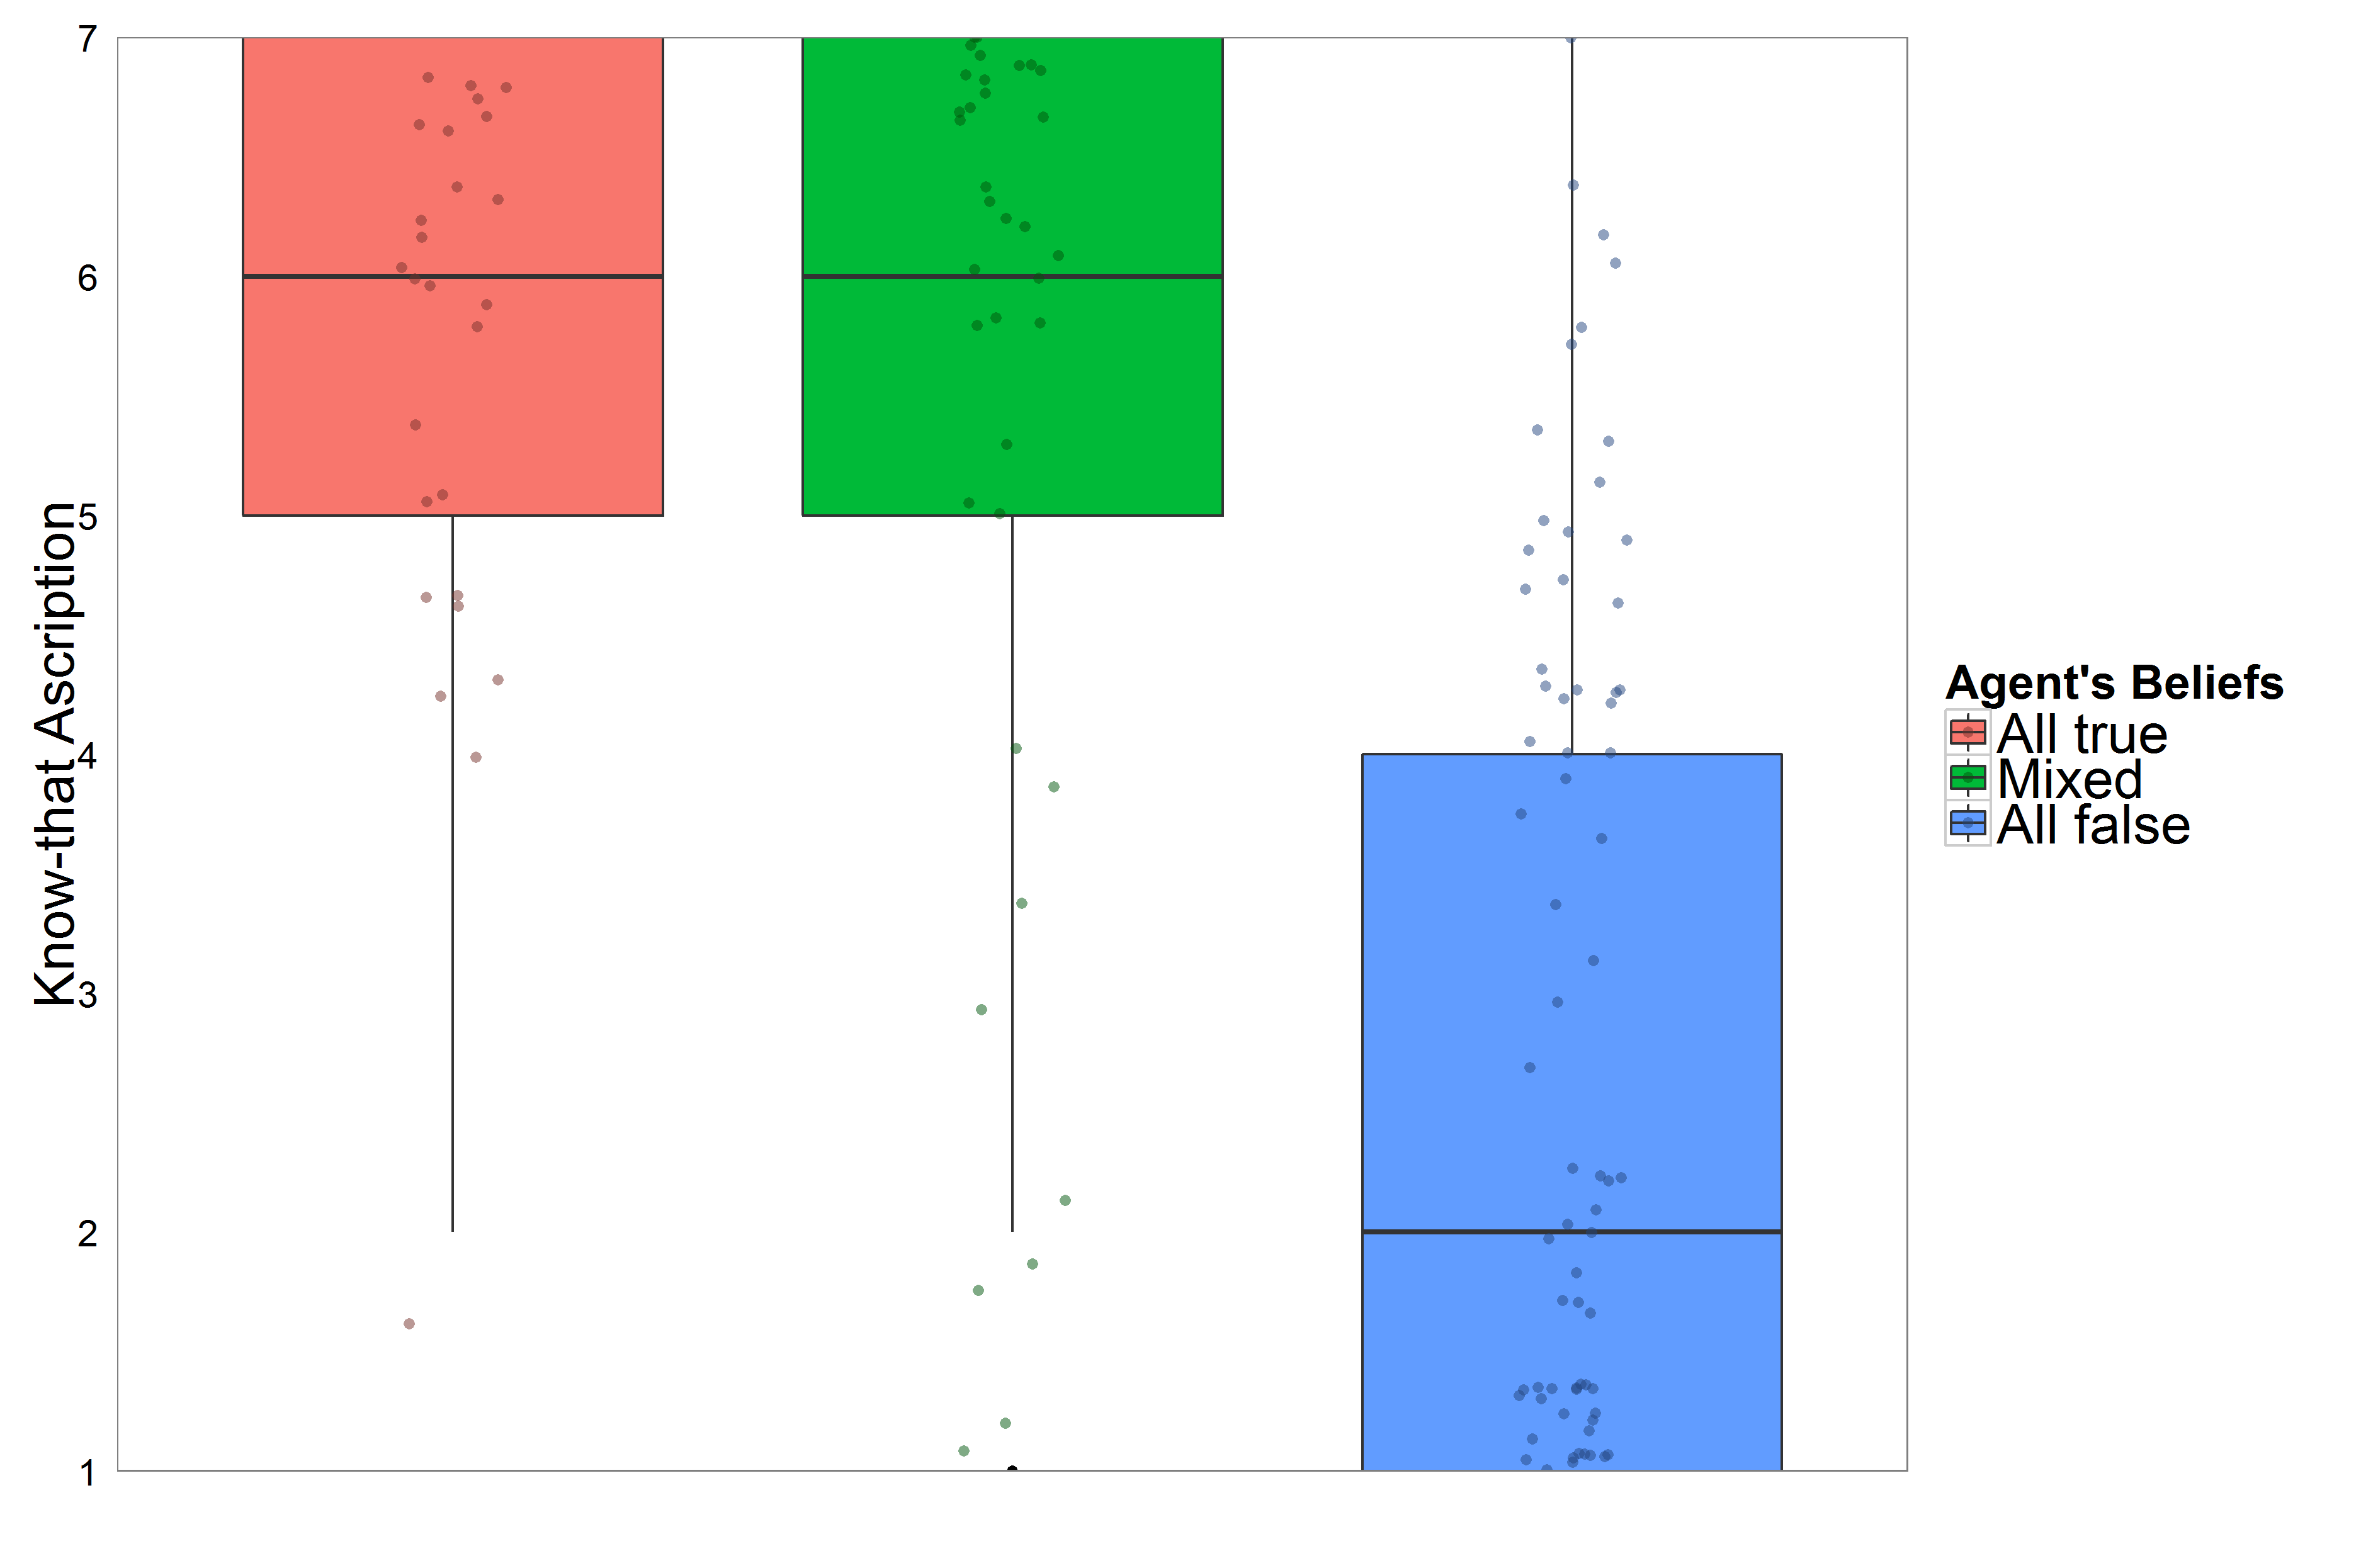
\includegraphics[width=14cm] {Fig3}
\captionsetup{width=0.9\textwidth}
\caption{Boxplots of participants' agreement rating with the knowledge that ascription in the \textbf{All True}, \textbf{Mixed} and \textbf{All False} conditions.}
\label{fig:Fig3}
\end{figure}

\subsection{Discussion}

While we saw above in Sections \ref{sec:study1} and \ref{sec:study2} that false beliefs are associated with degraded truth judgments for knowledge \textit{wh} ascriptions, we find no analogous effect for knowledge \textit{that} ascriptions. This suggests that we have a genuine challenge to accounts with the reducibility property: the different scenarios support the same facts regarding knowledge \textit{that}, suggesting that knowledge \textit{that} does not suffice to determine knowledge \textit{wh}.



\section{Experiment 4: The Naive Relevance-Implicature Approach}\label{implicatureTest}

In general, interest in the false-belief effect we have been investigating will hinge on how much it requires new or controversial theoretical machinery. In particular, to be a threat to reducibility (in anything like the sense considered by \citep{george:dis,george:thought} or \citet{kr:11}) it needs to be the case that belief in false answers compromises the \emph{truth} of the knowledge \textit{wh} ascription, rather than, e.g., producing a sentence that is true, but that, as a matter of something approximating classical Gricean post-compositional computation of conversational implicatures (cf.\ \citet{grice1975:logic}), is misleading in a way that renders a degraded truth judgment.\footnote{\citet{berman} is the most conspicuous advocate of an account of the false-answer effect along these lines.}

Our data show a number of gradability effects, and in particular show intermediate agreement ratings for most of the key cases. These intermediate agreement ratings make it tempting to try to write off the observed effect as this sort of implicature -- to say that \ref{sueknows} is straightforwardly semantically true in both the \textbf{All True} scenario and the \textbf{Mixed} scenario, but that in the latter it is infelicitous as the result of something akin to Gricean cooperative considerations.

\ex.[\ref{sueknows}]Sue knows where she can buy an Italian newspaper.

That is, we might say that the requirement that Sue not believe any false answers is not anything that presents a special challenge for the meaning of \textit{know} or for the question embedding construction.

There are, of course, numerous kinds of explanations along these lines, and we cannot attempt to evaluate all of them here. However, one family of these explanations seems especially intuitive (and is, in our experience, especially likely to be raised as a concern in discussions of these examples). Specifically, in reply to the judgments reported so far, a natural response would be to suggest that what is varying is the relevance of the knowledge facts to the implied problem-at-hand (with the \textbf{Mixed} scenario yielding degraded relevance and consequently degraded felicity). To flesh this out a bit, one of the main purposes served by knowledge reports is to identify people as information resources who can provide a solution for some problem. If (as is strongly suggested by the choice of example sentences and vignettes) the problem at hand is the problem of procuring an Italian newspaper, then, according to this line of reasoning, reporting that somebody knows where Italian newspaper can be bought should only be felicitous if this knowledge enables them to obtain Italian newspapers and to reliably direct others to places where they can buy such newspapers. Such an ascription would then suffer from degraded felicity in the \textbf{Mixed} case, arguably explaining away the reported judgment. 

In order to directly assess this line of analysis, we constructed a scenario in which knowledge is ascribed to a person who, although they know of a place where an Italian newspapers can be bought, is not a useful resource for solving the newspaper-obtaining problem at hand for reasons unrelated to false beliefs. We did this by varying whether the person to whom knowledge is ascribed shares a language in common with the person looking for a newspaper. If usefulness as a problem-solving resource is driving a relevance implicature effect responsible for these judgments, we should expect false beliefs and lack of a shared language to produce similar degraded truth judgments. If the judgments reported above are instead part of the conventional semantics of \textit{know wh}, we should expect the two cases to yield very different truth assessments.


\subsection{Methods}

257 (84 females, age $M( SD) = 29.53(9.12)$) participants with American IP addresses were recruited from Amazon's Mechanical Turk (www.mturk.com) and paid a small amount of money (\$0.35)in compensation for a small amount of their time ($<$ 7 minutes). Additional demographic information can be found in the supporting materials.

All participants read a vignette about a woman named Sue who wanted to know where she could buy an Italian newspaper and about a man named Bob who held beliefs about two stores which either did or did not sell Italian newspapers. To directly manipulate the relevance of the knowledge facts to the problem-at-hand (Sue's finding an Italian newspaper), we randomly assigned participants to read either a vignette in which Bob and Sue could not communicate because they did not share a common language \ref{sharedLang} or a vignette in which they could communicate because Bob and Sue did share a common language \ref{noSharedLang}. 

\ex.\label{sharedLang}Sue, who speaks only Italian and English, needs to buy an Italian newspaper. She is standing on the street near two stores: one called PaperWorld, and one called Cellulose City. Sue sees a man named Bob nearby. Bob is a native of the city who is normally very well-informed and trustworthy. \\ \\ Bob speaks only English and Hungarian. He believes that PaperWorld and Cellulose City sell Italian newspapers. He would be happy to tell this to Sue if she asked and he understood her. Moreover, Bob should be able to understand Sue's question, since they can speak the same language.  

\ex.\label{noSharedLang}Sue, who speaks only Italian and English, needs to buy an Italian newspaper. She is standing on the street near two stores: one called PaperWorld, and one called Cellulose City. Sue sees a man named Bob nearby. Bob is a native of the city who is normally very well-informed and trustworthy. \\ \\ Bob speaks only Cantonese and Hungarian. He believes that PaperWorld and Cellulose City sell Italian newspapers. He would be happy to tell this to Sue if she asked and he understood her. However, Bob would not be able to understand Sue's question, since they can't speak the same language.

Within each of these two conditions, participants were randomly assigned to read one of three possible cases: one in which Bob's beliefs about where to buy an Italian newspaper were all true \ref{s4allTrue}, on in which Bob's beliefs were both true and false \ref{s4mixed}, and one in which Bob's beliefs were all false \ref{s4allFalse}. 

\ex. 
\a. \label{s4allTrue} Bob is right about both stores: PaperWorld and Cellulose City both sell Italian newspapers.
\b. \label{s4mixed} Bob is right about PaperWorld. However, Bob is mistaken about Cellulose City, which does not sell Italian newspapers. (It is actually a stationery shop.)
\c. \label{s4allFalse} Bob is completely mistaken about PaperWorld and Cellulose City, neither of which sells Italian newspapers. (They are actually both stationery shops.)

After reading the vignette, participants rated their agreement with \ref{s4qK} on a scale from 1 (``Completely disagree'') to 7 (``Completely agree''). 

\ex. \label{s4qK} Bob knows where Sue can buy an Italian newspaper.

Subsequently, participants completed an item that was designed to measure the extent to which we were successful in manipulating the relevance-implicature \ref{felicityItem}. 

\ex. \label{felicityItem}Because Sue needs an Italian newspaper, she calls her friend Mary, to ask her what she should do, and happens to mention that she sees Bob nearby. Mary, who knows that Bob likes to keep up with the latest news from Italy, tells Sue \\ \\ ``Bob knows where you can buy an Italian newspaper.'' \\ \\ Given everything you know about Bob, how useful will Mary's information be to Sue?

Participants indicated their agreement on a scale from 1 (``Not at all useful'') to 7 (``Very useful''). Participants also completed two comprehension questions that simply asked whether they thought that Bob would understand Sue's question if she asked it in English and whether they thought it was likely that Sue would succeed in finding an Italian newspaper, given her situation. Lastly, participants answered a series of optional demographic items including whether English was their native language.

\subsection{Results}

8 participants were excluded because they did not indicate that English was their native language. An additional 16 participants were excluded for failing to correctly answer the first comprehension question.\footnote{The second comprehension question was not used to exclude participants because of an unforeseen lack of a clarity about what the ``correct'' answer was in some of the conditions. Regardless, the qualitative pattern of results remains the same even when not adopting any exclusion criteria.}

First, in order to ensure that we successfully manipulated the relevance of the knowledge \textit{wh} ascription by changing whether Bob and Sue shared a common language, we analyzed participants' judgments of how useful Mary's information was for Sue as indicated by their rating of \ref{s4qK}. A 2 (Language: Shared vs No Shared) $\times$ 3 (Belief: \textbf{All True} vs \textbf{Mixed} vs \textbf{All False}) Analysis of Variance (ANOVA), revealed a main effect of whether Bob and Sue shared a language, $F(1,227) = 42.04$, $p < .001$ $\eta_{p}^{2} = .156$, and a main effect of Belief State, $F(2,227) = 56.11$, $p < .001$ $\eta_{p}^{2} = .327$. Most importantly, though, we also observed a Language $\times$ Belief State interaction, $F(2,227) = 42.04$, $p < .001$ $\eta_{p}^{2} = .077$, which suggests that the impact of the truth of Bob's beliefs on judgments of usefulness differed when Sue and Bob shared a language and when they did not (see Fig. ~\ref{fig:Fig4}). Further investigation of this interaction effect revealed the predicted pattern of responses: when Sue and Bob shared a language, the usefulness of Mary's information was significantly affected by whether Bob's beliefs were all true (${M}({SD}) = 6.38(1.00)$) or were both true and false (${M}({SD}) = 5.15(1.51)$), $t(67.84) = 4.269$, $p < .001$, $d = 0.954$. However, when Sue and Bob did not share a language, the usefulness of Mary's information was no longer significantly affected by whether Bob's beliefs were all true (${M}({SD}) = 3.93(2.32)$) or were both true and false (${M}({SD}) = 3.46(1.80)$), $t(73.34) = 0.991$, $p = .325$, $d = 0.222$. Unsurprisingly, when Bob's beliefs were all false, Mary's information was never considered useful, regardless of whether Bob and Sue shared a language (${M}({SD}) = 2.36(1.76)$) or not (${M}({SD}) = 2.26(1.52)$), $t(69.23) = 0.256$, $p = .799$, $d = 0.060$.

\begin{figure}[h!]
\centering
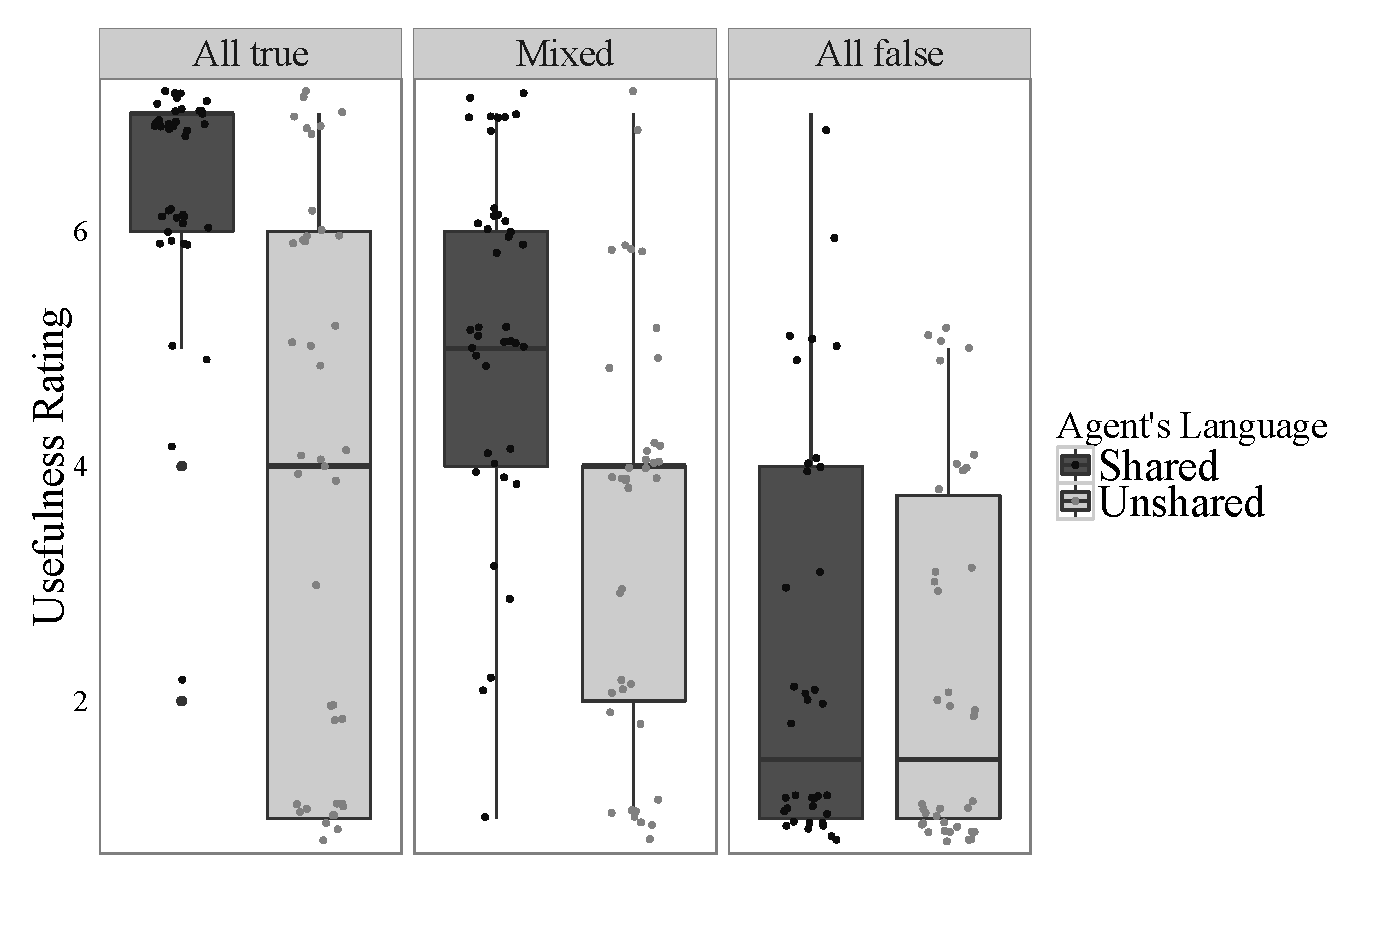
\includegraphics[width=14cm] {Fig4a}
\captionsetup{width=0.9\textwidth}
\caption{Boxplots of participants' ratings of the usefulness of the statement ``Bob knows where you can buy an Italian newspaper'' when Bob and Sue shared a language or did not share a language for the \textbf{All True}, \textbf{Mixed} and \textbf{All False} conditions.}
\label{fig:Fig4}
\end{figure}

The overall pattern of usefulness judgments allows us to appropriately test whether the difference in participants' agreement ratings with the knowledge \textit{wh} ascriptions can be adequately explained by the relevance of the knowledge facts to the implied problem-at-hand. If this relatively conservative, traditionally ``pragmatic'' line of analysis is correct, participants' agreement ratings with \ref{s4qK} should show a similar pattern such that the truth of Bob's beliefs affects participants' agreement with \ref{s4qK} when Bob and Sue share a language, but does not affect their agreement when Sue and Bob do not share a language, since the information is equally unhelpful in these latter cases.

To investigate whether this is the case, we next analyzed participants' agreement ratings with \ref{s4qK} (Fig. \ref{fig:Fig5}). A 2 (Language: Shared vs No Shared) $\times$ 3 (Belief: \textbf{All True} vs \textbf{Mixed} vs \textbf{All False}) ANOVA revealed a main effect of the truth of Bob's belief state, $F(2,227) = 256.17$, $p < .001$ $\eta_{p}^{2} = .693$, and a marginal effect of whether Bob and Sue shared a language, $F(1,227) = 3.58$, $p = .060$ $\eta_{p}^{2} = .016$. Critically, however, we did not observe a Language $\times$ Belief State interaction effect, $F(2,227) = 0.26$, $p = .773$ $\eta_{p}^{2} = .002$, which suggests that, unlike judgments of usefulness, agreement ratings with the knowledge \textit{wh} ascription were not differentially impacted by the falsehood of Bob's beliefs when Sue and Bob shared a language, compared to when they did not. Critically, even when Bob and Sue did not share a language, participants' agreed with the knowledge \textit{wh} ascription less when Bob had both true and false beliefs (${M}({SD}) = 5.21(1.69)$), than when Bob had all true beliefs (${M}({SD}) = 6.63(0.67)$), $t(49.34) = 4.89$, $p < .001$, $d = 1.111$. Similarly, when Bob and Sue shared a language, participants' agreed with the knowledge \textit{wh} ascription less when Bob had both true and false beliefs (${M}({SD}) = 4.90(1.63)$) than when Bob had all true beliefs (${M}({SD}) = 6.15(1.10)$), $t(68.39) = 4.89$, $p < .001$, $d = 0.899$. Moreover, comparing the two cases in which Bob has both true and false beliefs revealed that there is no significant difference in participants' agreement ratings with \ref{s4qK} when Bob and Sue share a language and when they do not $t(77) = -0.82$, $p = .416$, $d = 0.184$, suggesting that agreement with the knowledge \textit{wh} ascription in the \textbf{Mixed} cases was not significantly affected by the relevance of the knowledge facts to the implied problem at-hand.\footnote{A similar result is obtained when analyzing the data by comparing linear mixed models to test for three-way interaction which should be expected if the two different questions (knowledge \textit{wh} agreement vs. usefulness) are differentially sensitive to the interaction effect between the truth of Bob's beliefs and whether Bob and Sue shared a language. As predicted, we find evidence for the three-way interaction when comparing a model that includes the critical three-way interaction term (Judgment $\sim$ Question $*$ Language $*$ Belief State $+$ (1$|$Subject)) to one that does not contain that term (Judgment $\sim$ (Question $*$ Language) $+$ (Question $*$ Belief State) $+$ (Language $*$ Belief State) $+$ (1$|$Subject)), $\chi^2(1) = 19.937$, $p < .001$)}

\begin{figure}[h!]
\centering
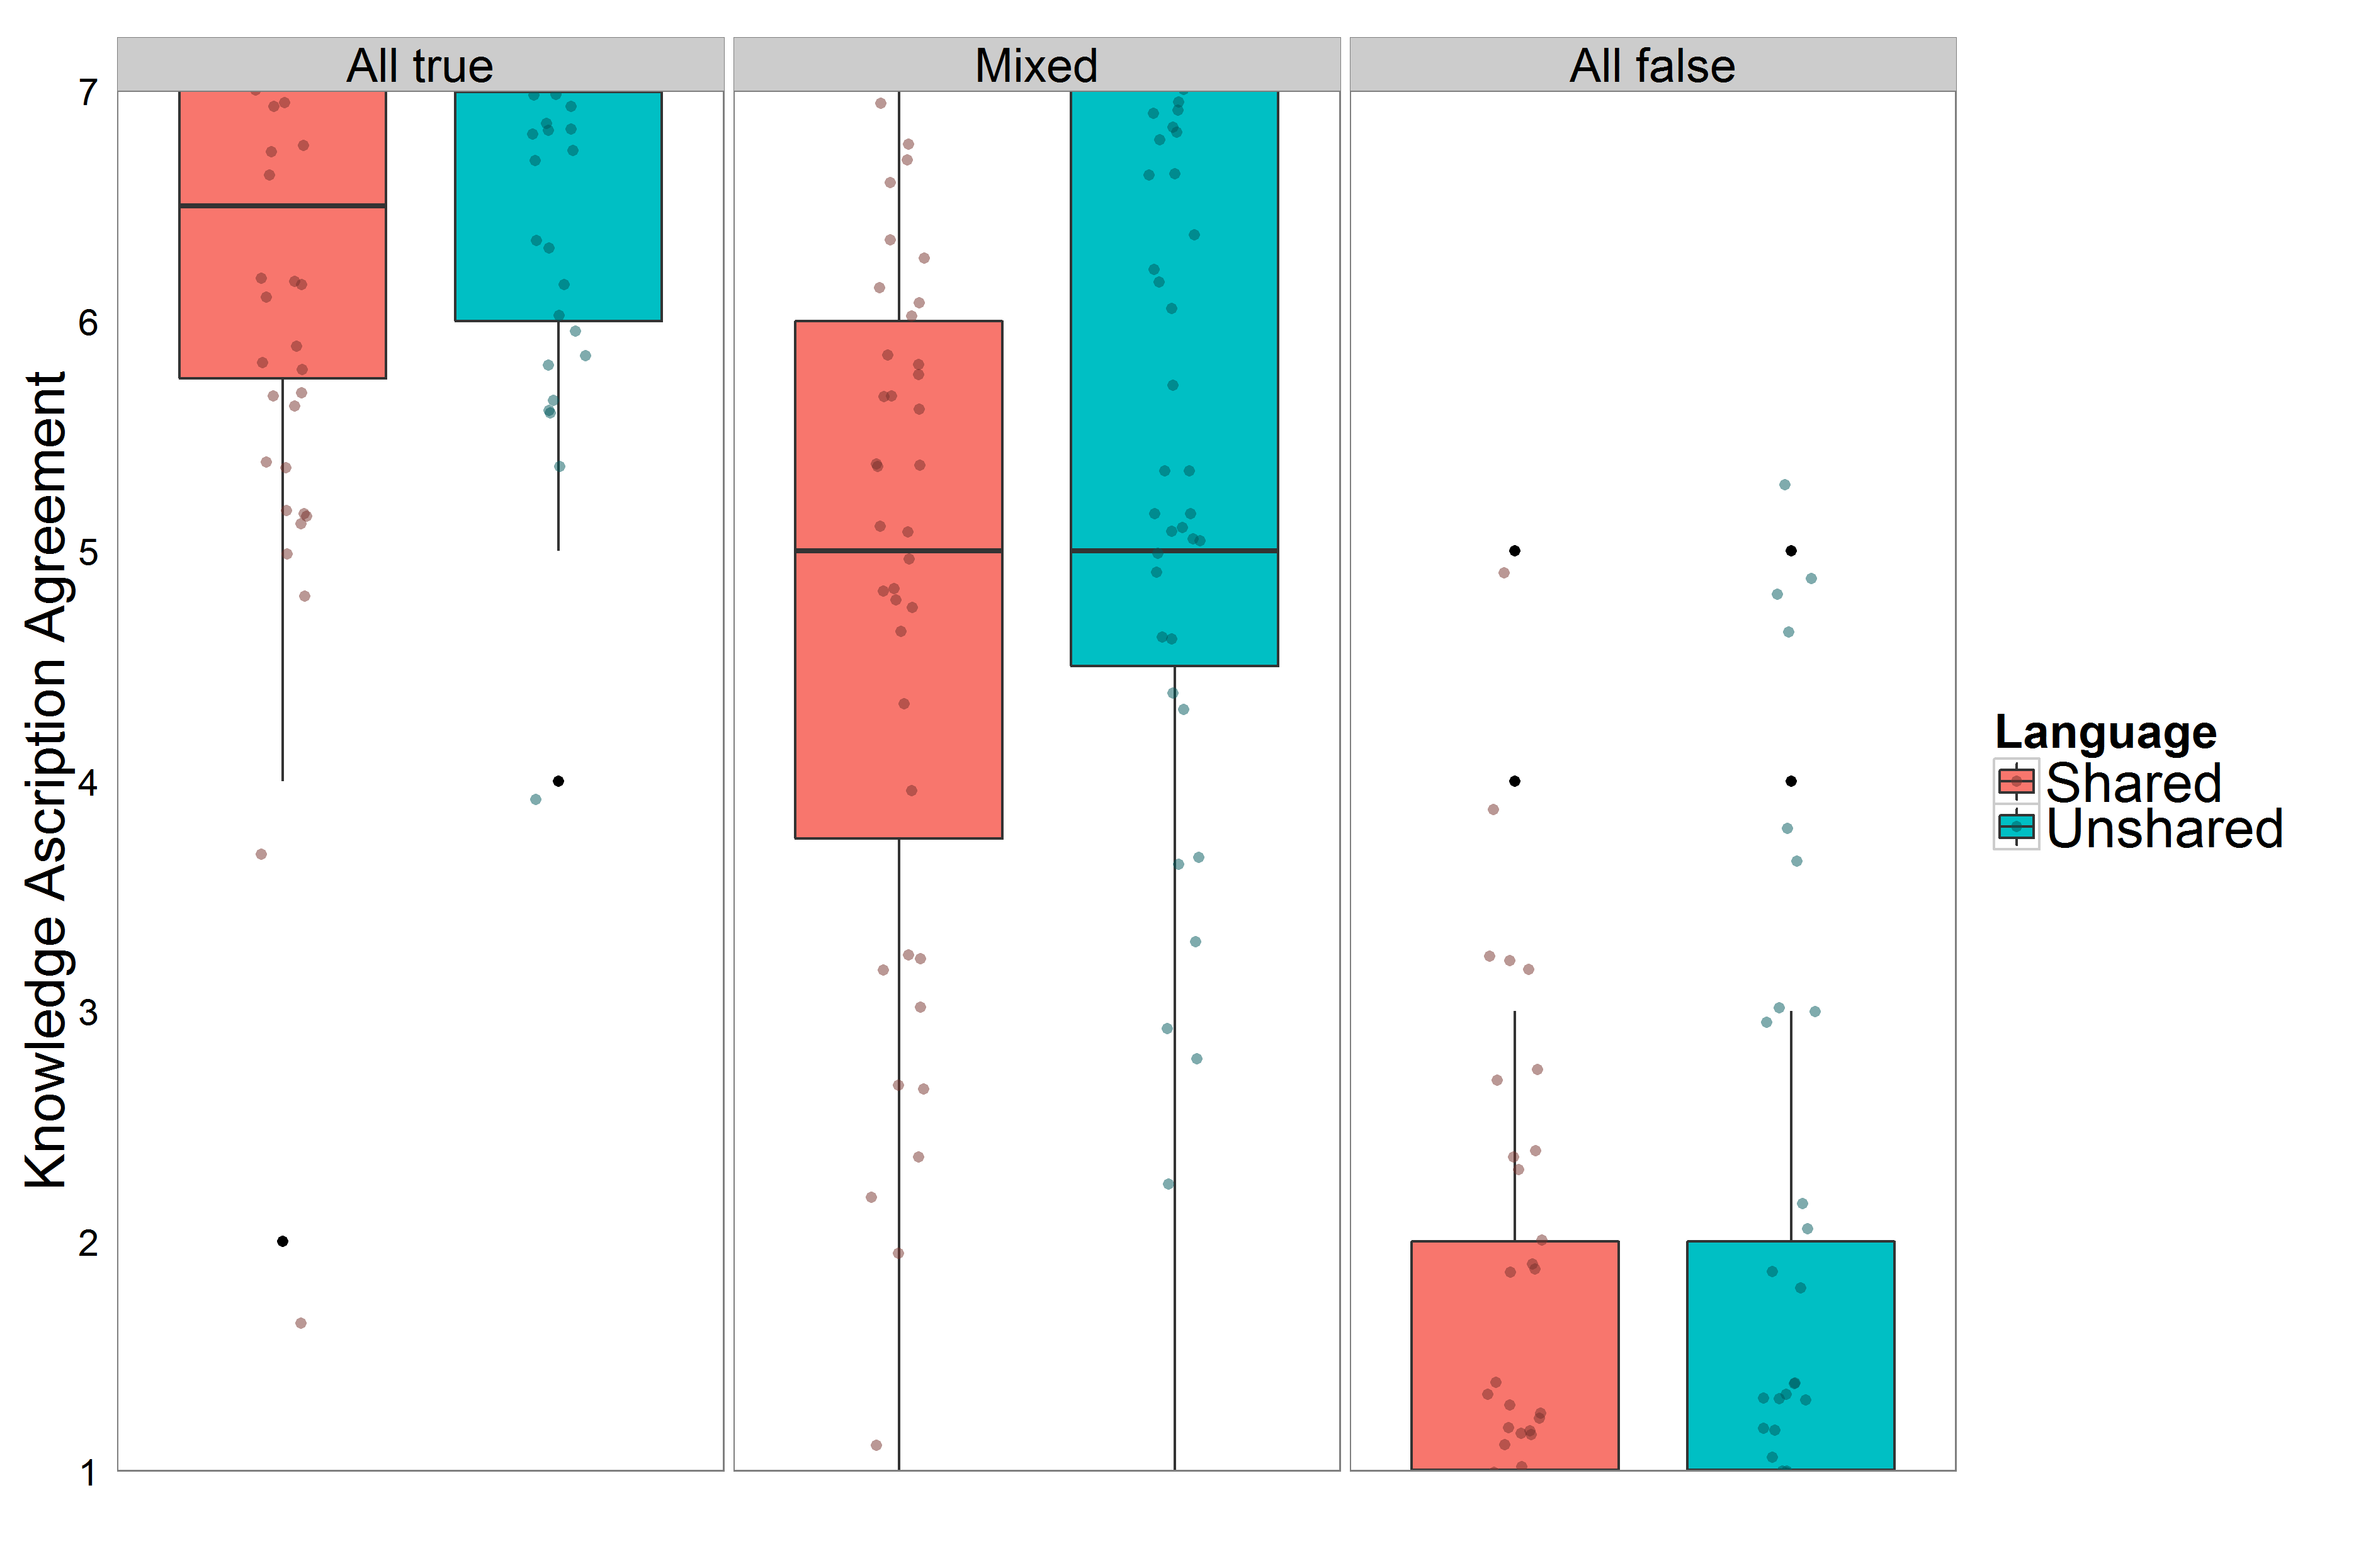
\includegraphics[width=14cm] {Fig4b}
\captionsetup{width=0.9\textwidth}
\caption{Boxplots of participants' agreement ratings with the knowledge \textit{wh} ascription when Bob and Sue shared a language or did not share a language for the \textbf{All True}, \textbf{Mixed} and \textbf{All False} conditions.}
\label{fig:Fig5}
\end{figure}


\subsection{Discussion}
These results count strongly against a classical Gricean relevance implicature analysis (or any similar relevance-driven analysis) of the key judgments for knowledge \textit{wh} ascriptions. When Bob's answer-knowledge is rendered irrelevant by a factor other than Bob's false beliefs (here a lack of a shared language), truth-judgments were not diminished, even though judgments of usefulness were. Thus, it would appear that false beliefs have some significance that goes beyond diminishing the relevance or utility of the underlying asnswer-knowledge facts and that, unlike relevance or utility, false beliefs diminishes truth status.

Alternative analyses along these lines deserve further investigation, and no one experiment will systematically rule out the possibility that the judgments that we've been discussing might admit of classical Gricean explication in a way that keeps false-belief sensitivity out of the lexicon and the operations of semantic composition. Still, these results help to put the burden of proof on the advocate of such an analysis. What we have seen so far is that the predictions of one very natural family approaches along these lines was not confirmed.\footnote{Of course, this experiment  does not resolve all questions about the kind of semantic or pragmatic meaning involved in false-belief sensitivity, and leaves open a variety of kinds of not-at-issue content, and more semantically entangled accounts that employ machinery that is ``pragmatic'' in the broad sense, such as those discussed by \citet{cremers:plurality} and \citet{xiang:sub:16}.} 

\section{Experiment 5: Who Knows How}

Thus far, we have focused on a \textit{know where} ascription that is familiar from the literature as an example of a mention-some reading for an embedded question (that is, a reading where partial information without false beliefs does not suffice to compromise the truth of the ascription). Naturally, it would also be important to see whether this effect extends to other kinds of knowledge \textit{wh}. In this section we consider \textit{know who} ascriptions (as another relatively widely-studied kind of knowledge \textit{wh}) and \textit{know how} ascriptions (which have received particular attention in discussions of reducibility in the philosophical literature, as in \cite{ryle:knowhow} and \cite{stanley:knowhow}).

\subsection{Methods}

364 (125 females, age (${M}({SD}) = 30.80(9.74)$) participants with American IP addresses were recruited from Amazon's Mechanical Turk (www.mturk.com) and paid a small amount of money (\$0.25) in compensation for a small amount of their time ($<$ 5 minutes). Additional demographic information can be found in the supporting materials. Participants either completed the ``knows how'' or ``knows who'' version of the study. 

In the ``knows how'' version, participants read a vignette that described a man named Jason who needs to know how to get to a hardware store because of a leaking pipe in his house \ref{knowsHow}. 

\ex. \label{knowsHow} Jason recently moved to a new town, and while he knows his way around the town, he doesn't know where the hardware store is. He needs to find a hardware store because there's a leaking pipe in his house. When Jason asks his neighbor where he can find a hardware store, his neighbor tells him that there's one four miles northeast and on the left side of the street. But when Jason asks his coworker where he can find a hardware store, his coworker tells him that there's one six miles south and on the right side of the street. Jason knows that his neighbor and his co-worker have lived in the town for about the same amount of time.

After participants read this vignette they were either told that all of Jason's beliefs were true \ref{s5allTrueH}, that they were both true and false \ref{s5mixedH}, or they were all false \ref{s5allFalseH}.

\ex. \label{s5allTrueH} There is a hardware store four miles northeast and on the left side of the street. There is also a hardware store six miles south and on the right side of the street.

\ex. \label{s5mixedH} There is a hardware store four miles northeast and on the left side of the street. There is no hardware store six miles south and on the right side of the street.

\ex. \label{s5allFalseH} There is no hardware store four miles northeast and on the left side of the street. There is also no hardware store six miles south and on the right side of the street.

After reading one of the three versions of this vignette, participants rated their agreement with \ref{s5qKh}.

\ex. \label{s5qKh} Jason knows how to get to a hardware store. 

The ``knows who'' version was similarly structured. Participants read a vignette that described a woman named Amy who needs to know \emph{who} has a MiniDisplayPort adapter so that she can connect her computer to a projector. Amy's friend Bert tells her that two different coworkers have the adapter she needs. Similar to the ``knows how'' version, Amy's beliefs could have all been true, have been both true and false, or all have been false. Participants were randomly assigned to one of these three conditions. We also included an additional condition to ensure that this vignette correctly elicited a mention-some reading.\footnote{Analogous tests were not included for other ascriptions because they represent cases where the availability of a mention-some reading is already widely assumed in the literature and is, as far as we know, not in serious dispute. In contrast, our \emph{know who} sentence does not correspond directly to any standard mention-some example in the literature.} In this version, Amy has only true beliefs about who has a MiniDisplayPort adapter, but is ignorant of an additional coworker who also has the adapter she needs. After reading the vignette, all participants rated their agreement with \ref{s5qKw}. 


\ex. \label{s5qKw} Amy knows who can lend her an adapter. 

In both versions of the study, participants rated their agreement on a scale from 1 (``Completely disagree'') to 7 (``Completely agree''). Additionally, participants who read about Amy answered a comprehension question which asked them to indicate which of Amy's coworkers actually had the adapter that Amy needed. This question was only included in the know \textit{who} version because of the relative complexity of the scenario. Finally, all participants answered a series of optional demographic items including whether English was their native language.

\subsection{Results}

16 participants were excluded because they did not indicate that English was their native language. An additional 21 participants were excluded because they did not correctly answer the comprehension question in the ``knows who'' version. An analysis of the mention-some test for the ``knows who'' version revealed that participants mean agreement with \ref{s5qKw} was significantly above the midpoint of 4 (${M}({SD}) = 5.67(1.37)$), $t(44) = 8.19$, $p < .001$, $d = 1.22$ suggesting that a mention-some reading was clearly available in the knows who case. Accordingly, we proceeded to consider whether knowledge \textit{wh} truth assessments were affected by the truth of the agents' beliefs.

The primary 2 (Knowledge-\textit{wh} ascription: who vs how) $\times$ 3 (Beliefs: \textbf{All True} vs \textbf{Mixed} vs \textbf{All False}) analysis of variance of the remaining 282 participants' agreement ratings revealed that their agreement was significantly influenced by the truth of the agent's beliefs $F(2,276) = 130.33$, $p < .001$ $\eta_{p}^{2} = .482$ (Fig. \ref{fig:Fig6}). Most importantly, participants agreed with the knowledge ascriptions more when the subjects beliefs were all true (${M}({SD}) = 5.61(1.72)$) than when they were both true and false (${M}({SD}) = 4.15(1.89)$), $t(184.18) = 5.50$, $p < .001$, $d = 0.802$. In addition, in the ``knows who'' \textbf{Mixed} condition, participants' agreement was also significantly lower (${M}({SD}) = 4.64(1.96)$) than their agreement in the additional ``knows who'' mention-some test, where the agent was simply ignorant of relevant answer knowledge rather than having a false belief $t(72.64) = -2.81$, $p = .006$, $d = 0.610$.

We additionally observed an unpredicted main effect such that participants were overall more willing to agree with the knowledge ascription in ``knows who'' version (${M}({SD}) = 4.46(2.34)$) than in the ``knows how'' version (${M}({SD}) = 3.39(2.12)$), $F(1,276) = 27.10$, $p < .001$ $\eta_{p}^{2} = .089$. While this difference was not anticipated, it is relatively unsurprising given the number of differences between the ``knows who'' and ``knows how'' vignettes. More  importantly, we did not observe a significant interaction effect $F(1,276) = 2.85$, $p = .060$ $\eta_{p}^{2} = .020$, suggesting that the agent's false beliefs had at least a somewhat similar impact of both types of knowledge \textit{wh}.
    
\begin{figure}[h!]
\centering
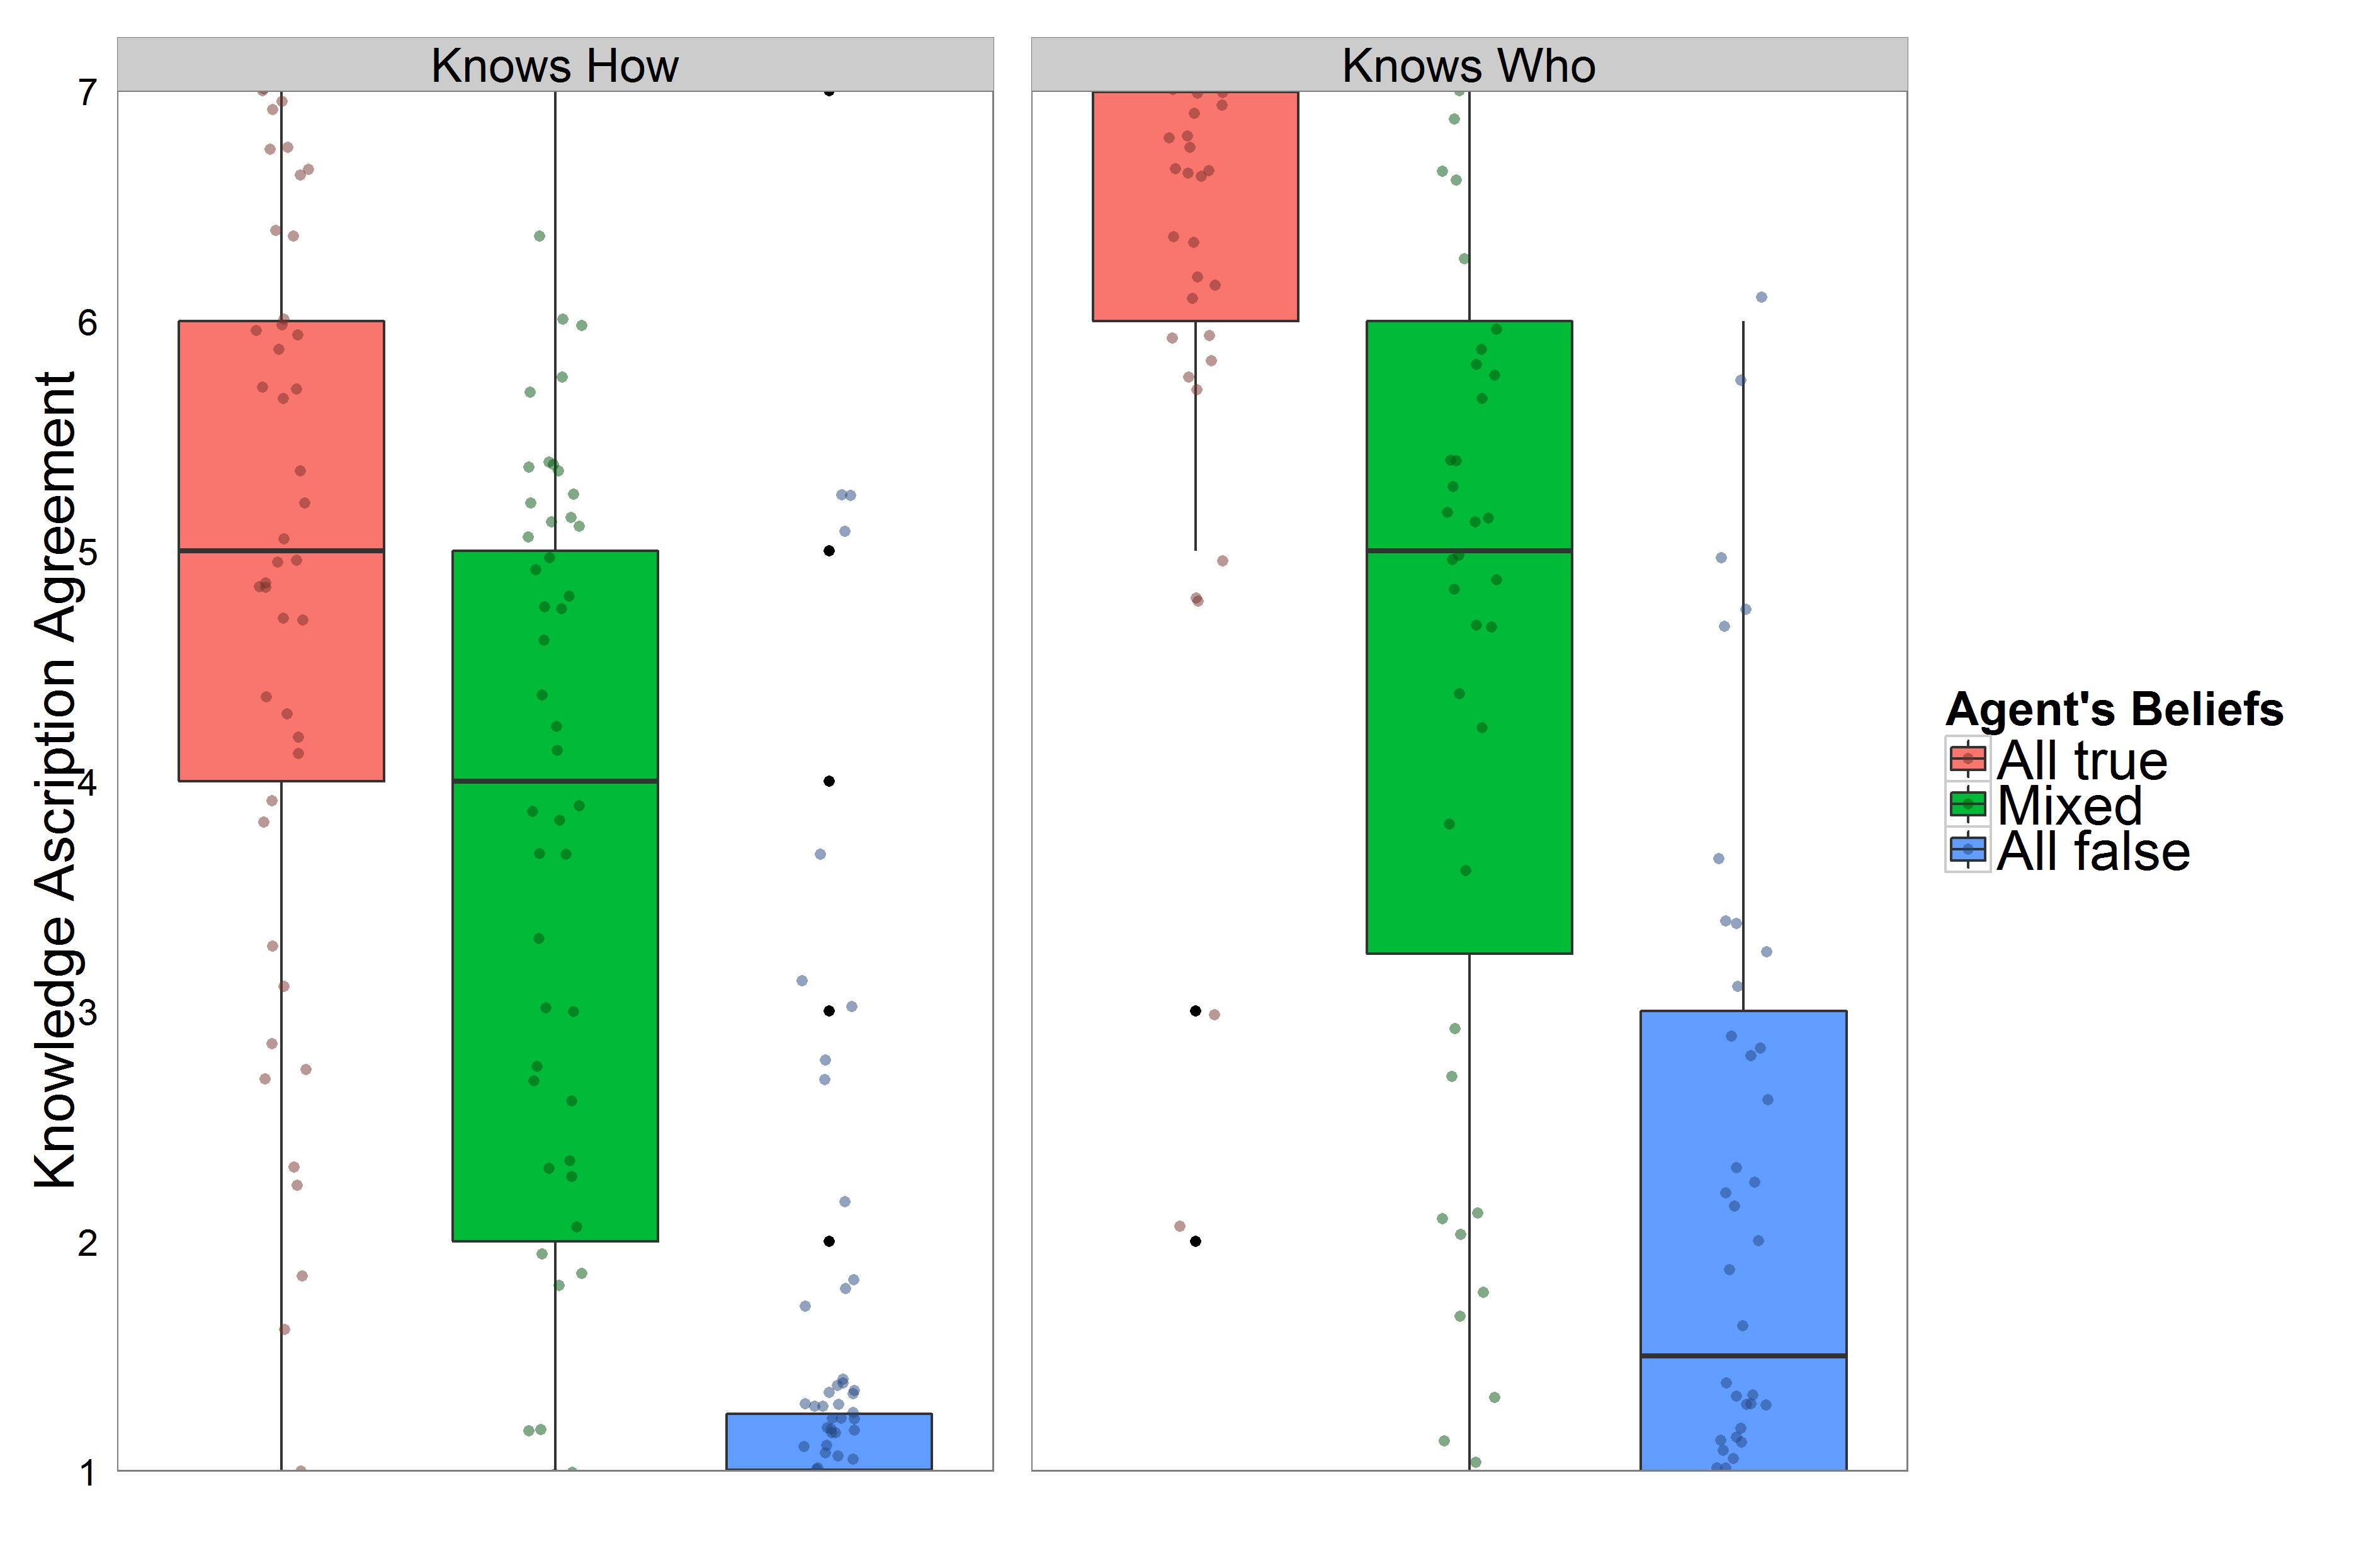
\includegraphics[width=14cm] {Fig5}
\captionsetup{width=0.9\textwidth}
\caption{Boxplots of participants' agreement ratings with the knowledge \textit{wh} ascription in the \textbf{All True}, \textbf{Mixed} and \textbf{All False} conditions for \textit{knows how} (left) and \textit{knows who} (right).}
\label{fig:Fig6}
\end{figure}

\subsection{Discussion}

These results indicate that the effect we observe is replicated in a variety of types of \textit{wh} questions, including the \textit{who} questions that are often used as the standard case in work on \textit{wh} questions semantics, and the \textit{how} questions that have received special attention in philosophical work on reducibility \citep{ryle:knowhow,stanley:knowhow}. Given the similarity of the pattern observed here to the pattern observed throughout the four preceding studies, there is good reason to think that this effect applies quite generally to knowledge \textit{wh}. Taken together, these five studies provide robust support for the non-reducibility of knowledge \textit{wh}.

\section{Experiment 6: Proportion-Sensitivity}\label{proportionalsec}

The previous studies were informative in demonstrating \textit{that} false beliefs affect truth assessments of knowledge \textit{wh} ascriptions, they are not particularly informative as to \textit{how} false beliefs affect participants' truth assessments. At a level of descriptive claims, most semantic treatments of false-belief sensitivity in knowledge \textit{wh} follow \citet{spector:05} (for mention-all readings) or \citet{george:dis} (for mention-some readings).\footnote{This is true at least as far as false positive beliefs are concerned. The most notable departure from the overall descriptive picture is exemplified by \citet{xiang:sub:16}, who describes a sensitivity to false negative beliefs as well as false positive beliefs, but agrees with the standard picture as far as the impact of false positives is concerned.} On this picture, a single false positive belief defeats the truth of a knowledge \textit{wh} claim. This descriptive picture, especially in the mention-some case, was derived from a small number of judgments for vignettes and examples like those above, where only two potential answers are involved. 

Thus far, the empirical data we have presented suggest degraded truth judgments in these cases, but do not pattern with clear at-issue falsehood (although we have not yet identified an unproblematic alternative). In discussions of the alleged descriptive pattern with other philosophers and linguists, it has been our informal impression that those who endorse false-belief sensitivity in truth-value judgments are more inclined to focus on scenarios with a higher proportion of false to true beliefs, while those who reject false-belief sensitivity are more inclined to focus on scenarios with a higher proportion of true to false beliefs (e.g., a person who would happily name 100 stores that sell Italian newspapers, 99 of which in fact do).

These points together suggest to us that the descriptive space of judgments for these proportions is both under-explored and worth exploring. As a first step to addressing this issue, we designed a final experiment that allowed us to come slightly closer to parametrically varying the proportion of the agent's beliefs that were false, which allowed us to begin to measure how participants' truth assessments of knowledge \textit{wh} ascriptions vary as function of the increasing proportion of false beliefs. For comparison, we additionally collected assessments of knowledge \textit{that} ascriptions.\footnote{We'd like to thank an anonymous reviewer at Journal of Semantics for this suggestion.} 

\subsection{Methods}

For knowledge \textit{wh} assessments, 171 (46 females, age (${M}({SD}) = 29.61(9.83)$) participants with American IP addresses were recruited from Amazon's Mechanical Turk (www.mturk.com). For knowledge \textit{that} assessments, an additional 200 (99 females, age (${M}({SD}) = 34.59(11.76)$) participants with American IP addresses were recruited. Participants were paid a small amount of money (\$0.25) in compensation for a small amount of their time ($<$ 5 minutes). Additional demographic information can be found in the supporting materials.

All participants read a vignette in which a woman named Sue was told where to buy a newspaper by her friend Bob \ref{s6prop}. 

\ex. \label{s6prop} Sue is standing on the street near three stores: one called PaperWorld, one called Cellulose City, and one called Newstopia. Sue's friend, Bob, a native of the city who is normally very well-informed and trustworthy, told her that PaperWorld, Newstopia, and Cellulose City all sell Italian newspapers. Having no reason to doubt this, Sue has always assumed that Bob was right. 

Participants were told that Bob was either correct about all three stores \ref{s63-0}, correct about two of the three stores \ref{s62-1}, correct about only one of the stores \ref{s61-2}, or incorrect about all of the stores \ref{s60-3}.

\ex. \label{s63-0} Bob was correct about all three stores, which do in fact all sell Italian newspapers.

\ex. \label{s62-1} However, Bob completely misinformed Sue about PaperWorld, which does not sell newspapers, but is actually a stationery shop. Bob was correct about Newstopia and Cellulose City.

\ex. \label{s61-2} However, Bob completely misinformed Sue about PaperWorld and Cellulose City, which do not sell newspapers, but are actually both stationery shops. Bob was correct about Newstopia.

\ex. \label{s60-3} However, Bob completely misinformed Sue about all three stores, none of which sell Italian newspapers. PaperWorld and Cellulose City, are actually both stationary shops, and Newstopia is an ironically misnamed shop that sells T-shirts with obnoxious political slogans.

Participants recruited to assess knowledge \textit{wh} ascriptions rated their agreement with \ref{sueknows}, as in previous studies. Participants recruited to assess knowledge \textit{that} ascriptions instead rated their agreement with \ref{s3qa}

\ex.[\ref{sueknows}]Sue knows where she can buy an Italian newspaper. 

\ex.[\ref{s3qa}]Sues knows that she can buy an Italian newspaper at Newstopia.

Finally, participants were asked to summarize the story they read and then to complete a series of optional demographic items including a question asking whether English was their native language. For this study, and all of the preceding studies, all stimuli, data, analyses, and other supporting materials can be retrieved from: \url{https://github.com/phillipsjs/Knowledge_wh}.

\subsection{Results}

First, the data were combined to allow for an overall analysis including both Belief Condition and Ascription Type. We excluded 8 participants because they did not indicate that English was their native language. Agreement ratings from the remaining participants revealed a main effect of the type of knowledge ascription, $F(1,355) = 45.28$, $p < .001$, $\eta^2 = .113$, a main effect of belief condition, $F(3,355) = 67.73$, $p < .001$, $\eta^2 = .361$, and, most critically an Ascription Type $\times$ Belief Condition interaction effect, $F(3,355) = 8.10$, $p < .001$, $\eta^2 = .064$. We further investigated this interaction by separately considering the effect of belief condition on each type of knowledge ascription. 

Participants' assessments of knowledge \textit{that} ascriptions revealed an overall effect of Belief Condition $F(3,191) = 23.81$, $p < .001$, $\eta^2 = .272$ (Fig. \ref{fig:Fig7}). However, this effect was completely driven by comparative disagreement in the condition where Newstopia did not actually sell newspapers. That is, participants only disagreed that Sue knew that she could buy an Italian newspaper at Newstopia when Newstopia did not in fact sell Italian newspapers, ${M}({SD}) = 3.63(2.50)$.\footnote{The high amount of variance in the answers to this question is likely due to the presupposition failure suffered by \ref{s3qa} in this condition.} In all of the other conditions, in which Newstopia did sell newspapers, participants' agreement with \ref{s3qa} was not significantly affected by the number of Sue's beliefs that were false, $F(2,146) = 2.17$, $p = .118$, $\eta^2 = .029$.

Critically, participants' assessments of knowledge \textit{wh} ascriptions also revealed an effect of Belief Condition $F(3,164) = 52.74$, $p < .001$, $\eta^2 = .491$ (Fig. \ref{fig:Fig7}). In this case, however, the pattern of participants' assessments was substantially different. Participants agreed most strongly with \ref{sueknows} when Sue's beliefs were all true (${M}({SD}) = 6.17(1.39)$), somewhat less when one of Sue's beliefs was false (${M}({SD}) = 5.31(1.69)$), even less when two of Sue's beliefs were false (${M}({SD}) = 3.77(2.01)$), and least of all when Sue's beliefs were all false (${M}({SD}) = 1.88(1.60)$). In each case, the presence of an additional false belief significantly reduced participants' agreement ratings (\textit{p}'s $< .05$; $d$'s $> .56$).

\begin{figure}[h!]
\centering
\includegraphics[width=14cm] {Fig6_revision}
\captionsetup{width=0.9\textwidth}
\caption{Agreement rating with the knowledge \textit{wh} ascription as a function of the portion of the agent's beliefs that were false.}
\label{fig:Fig7}
\end{figure}

\subsection{Discussion}

As these results demonstrate,  truth assessments of knowledge \textit{wh} ascriptions are sensitive not only to the mere presence of false beliefs but also to the proportion of the agent's question-relevant beliefs that are false. Moreover, participants on average disagreed with the knowledge \textit{wh} ascription when the agent had proportionally more false beliefs than true beliefs. Importantly, this pattern was observed in a context in which the knowledge \textit{that} facts remain unchanged. Such results both provide strong support for some form of non-reducibility and require an account of knowledge \textit{wh} with the resources to handle the sort of proportionality effect demonstrated here. 

\section{Theoretical Implications and Interpretation}

The observations presented here suggest that there is a false-belief effect for knowledge \textit{wh}. Although they do not resolve its precise status among the range of notions of semantic and pragmatic meaning, our results help to narrow things down. Specifically, they undermine traditional treatments of knowledge \textit{wh} ascriptions, and support the claim that, with mention-some questions, knowledge \textit{wh} is not (in the strictest sense) reducible of knowledge \textit{that} (whether it might be reducible in some looser sense will depend on some details of one's theoretical perspective).

These observations help somewhat to flesh out the picture of false-answer effects and support a claim of non-reducibility for knowledge \textit{wh}. For a variety of types of questions, we find that we can get something like mention-some truth conditions in the absence of false beliefs, together with decreased truth-value agreement in the case where there are additional false beliefs. This seems to be a genuine challenge to answer-based reducibility, as the introduction of false beliefs does not have a corresponding change on truth-value judgments of knowledge \textit{that} ascriptions for answers. Moreover, we find that the diminished agreement pattern seen in these cases is not found in cases where there are only true beliefs, but where relevance or utility of the statement is otherwise compromised, suggesting that the most obvious classical Gricean implicature treatment cannot straightforwardly ``explain away'' this effect. (This of course does not preclude many other kinds of accounts that are ``pragmatic'' in some broader sense.)

Although we think our observations clearly count against some existing approaches, it is much less clear what the correct positive account of knowledge \textit{wh} should look like. In particular, the most common descriptive generalizations fail to capture many of our observations. Most of the accounts of false-belief sensitivity available appeal to a ``no false beliefs'' requirement: they require some amount of knowledge of true answers (for the cases studied here, knowing a single \emph{mention-some answer} suffices), without belief in any false answer. 

Contrary to this all-or-nothing picture, we find that cases involving false belief produce an intermediate agreement rating that is distinct from judgments in cases of clear falsehood -- suggesting either that the false-belief effect operates at some level of not-at-issue meaning, or that it admits of some kind of intermediate case. Further, contrary to the standard characterization of false-belief sensitivity as a ``no false beliefs'' requirement, we find that	 the level of agreement deteriorates monotonically with the proportion of known answers to false beliefs -- an effect which is completely unexpected on standard pictures of false-belief sensitivity.

Our observations suggest that established accounts will need to be adjusted to allow for some way of capturing graded agreement with knowledge \textit{wh} ascriptions. One natural way of accounting for gradable truth judgments like those seen in Section \ref{proportionalsec} is to treat them as some sort of borderline case. We might, following the general spirit of many popular semantic treatments of borderline cases and related types of gradability, say that there is some threshold proportion of true beliefs sufficient for truth of the knowledge \textit{wh} ascription, but that this threshold is determined by a flexible parameter -- say, a contextual parameter that may be underspecified or allows for accommodation, as is common of contextual parameters.

The exact choice of formal implementation is not critical here, but, to get a sense of how this would work, consider canonical examples of quantifiers like \textit{many} or \textit{enough} that readily admit of the right sort of contextual flexibility. Clearly, these quantifiers admit borderline cases, where we would both be reluctant to unequivocally claim that there were ``enough $X$s'', and also reluctant to unequivocally claim that there were ``not enough $X$s''. They also exhibit context-sensitivity: the criteria for satisfying them depend, among other things, on the standard of numerousness or sufficiency at hand in the conversational context.

One way of handling this kind of phenomenon in a classical bivalent semantics is to analyze \textit{enough} as something like \textit{more than $t$}, where the exact value of the threshold $t$ is not clearly fixed by the lexicon, but is allowed to vary with conversational context in a way that allows it to be sensitive to the task at hand or the topic of interest. The complete details of \textit{enough} are of course considerably more complex, but this notion of sensitivity to a contextually supplied threshold or standard is found in analyses of many phenomena, and it allows us to analyze intermediate truth/agreement judgments as representing hearer's reluctance, but not flat-out unwillingness, to consider a value of this contextual variable that would make the sentence under consideration true.

Thus, while most false belief-sensitivity accounts of knowledge \textit{wh} give \ref{knowbasic} truth conditions equivalent (or nearly equivalent) to the conjunction of \ref{knowexist} and \ref{knowall}, our observations about proportion-sensitivity suggest that we might do better to analyze it by conjoining \ref{knowexist} with something like \ref{knowmany}, \ref{knowenough}, or \ref{knowpercent}. That is, it seems preferable to analyze it in terms of some fuzzier, more standard-dependent requirement on avoiding false beliefs, rather than the absolute prohibition on false belief.

\ex.\label{knowbasic} John knows where he can buy an Italian newspaper.

\ex.\label{knowexist} There is $x$ s.t.\ J.\ knows he can buy an Italian newspaper at $x$.

\ex.\label{variouscriteria}\a.\label{knowall} For every $x$ s.t.\ J.\ believes he can buy an Italian newspaper at $x$, he in fact can.
\b.\label{knowmany} For many $x$ s.t.\ J.\ believes he can buy an Italian newspaper at $x$, he in fact can.\\(Where the amount that constitutes many is in part determined by conversational context.)
\b.\label{knowenough} For enough $x$ s.t.\ J.\ believes he can buy an Italian newspaper at $x$, he in fact can.\\(Where the threshold that determines enough is in part determined by conversational context.)
\b.\label{knowpercent} For more than $n\%$ of the $x$ s.t.\ J.\ believes he can buy an Italian newspaper at $x$, he in fact can.\\(Where $n$ is a contextually supplied threshold.)

The intermediate agreement would then reflect differences among speakers about the standard or other parameters involved in the evaluation of \ref{knowmany}, \ref{knowenough}, or \ref{knowpercent}, as well as uncertainty on the part of individual speakers regarding how these standards should be set.

The above are obviously not complete or fully-satisfying proposals, but they call attention to the way that these types of gradability and context  sensitivity are widespread, and not in any way special to knowledge \textit{wh}. Approaches along these lines all yield a false-belief effect, and are all problematic for reducibility, but still vary considerably in their details.

\section{Open Problems}

Our present empirical investigation suggests that truth judgments for knowledge \textit{wh} are affected by false beliefs, and that this gives rise to a pattern of judgments incompatible with the standard picture of the relationship between knowledge \textit{that} and knowledge \textit{wh}, and with reducibility more generally. 

Still, we have left many issues unresolved. It is not clear exactly what the role of false belief is in these examples. The results in Section \ref{proportionalsec} takes one small step toward fleshing out the picture, but the various partly degraded truth-value judgments are, as already noted, difficult to account for with the tools typically employed in the formal semantics of question embedding. A full positive account of knowledge \textit{wh} is still needed, and more theoretical and empirical work will be needed to fill out the details of such an account.

We have also not looked beyond \textit{know} to other attitudes. Numerous other propositional attitude predicates can embed questions, and some of these may may give rise to non-reducibility effects,\footnote{\cite{george:dis} suggests \textit{forget} as a likely candidate -- see there, \citet{kr:11}, and \citet{cg:15} for discussion of a few other possibilities.} false-answer sensitivity,\footnote{See \citet{berman,heim:94,kr:11,preuss} for some for some plausible examples.} or both. Similar effects with other attitudes are possible and deserve to be explored. It would also be desirable to produce some general theory of question embedding, and of the relationship between propositional and question-oriented uses of an embedder. Ideally, such an account would identify what is uniform across different embedders, and which degrees of freedom are available: if reducibility must be rejected, we should have some story of what takes its place as the link between attitudes \textit{that} and attitudes \textit{wh}.

Many accounts for this are available, but few provide a reasonable level of uniformity while allowing for the full range of false-answer and non-reducibility effects, and none of these have, to our knowledge, incorporated a satisfying solution to the proportion sensitivity seen in our last experiment. These remain important issues for future research.

\bibliography{questionbib3a}

%\theendnotes

\end{document}